\documentclass[conference]{IEEEtran}
\IEEEoverridecommandlockouts
\usepackage{cite}
\usepackage{multirow}
\usepackage{algorithm}
\usepackage{algpseudocode}
\usepackage{lipsum}
\usepackage{adjustbox}
\usepackage{booktabs}
\usepackage{amsmath,amssymb,amsfonts}
\usepackage{makecell}
% \usepackage{algorithmic}
\usepackage{array}
\usepackage{listings}
\usepackage{graphicx}
\usepackage{hyperref}
\usepackage{textcomp}
\usepackage{amsthm}
\usepackage{tabularx}
\theoremstyle{definition}
\newtheorem{definition}{Definition}
\newtheorem{exmp}{Example}
\usepackage{float}
\usepackage{enumitem} 
\usepackage[most]{tcolorbox}
\usepackage{url}
\usepackage[table,xcdraw]{xcolor}
\usepackage{xspace}
\usepackage{amssymb}
\usepackage{tikz}
\usepackage{flushend}
\usepackage{threeparttable}
\usepackage{algorithmicx}
\newcommand{\circlednum}[1]{%
  \tikz[baseline=(char.base)]{
    \node[shape=circle,draw,inner sep=0.5pt] (char) {#1};
  }
}
% 自定义命令，根据输入的值生成颜色
\newcommand{\colorvalue}[1]{%
    \pgfmathsetmacro{\value}{#1}%
    \pgfmathsetmacro{\colorIntensity}{(\value-0.5)*100}% 将0.5-1.0的范围映射到0-100的颜色强度
    \cellcolor{blue!\colorIntensity} #1
}

\newtcolorbox{simplebox}[2][]{colframe=blue!50!black, colback=blue!10, boxrule=0.4mm, arc=3mm, #1}

\setlist[enumerate]{nosep, leftmargin=*, align=left} 

\usepackage{tabularx} 
\def\BibTeX{{\rm B\kern-.05em{\sc i\kern-.025em b}\kern-.08em
    T\kern-.1667em\lower.7ex\hbox{E}\kern-.125emX}}
\begin{document}

\newlist{inlineenum}{enumerate*}{1} 
\setlist[inlineenum]{
  label=\alph*), 
  itemjoin=\quad,  
  before={}, 
  after={}
}

\newcommand{\kg}{\textit{KubeGuard}\xspace}
\newcommand{\kger}{\textit{KubeGuarder}\xspace}

\title{\kg: A Systematic Permission-Oriented Risk Detection Approach for Kubernetes Applications\\

%\thanks{*Corresponding author: Chang-ai Sun (casun@ustb.edu.cn)}
}

% \author{\IEEEauthorblockN{Chang-ai Sun*,Yu-fei Gong,Xiao-yang Han}
% \IEEEauthorblockA{\textit{School of Computer and Communication Engineering} \\
% \textit{University of Science and Technology Beijing}\\
% Beijing, China \\}
% \and
% \IEEEauthorblockN{Huai Liu}
% \IEEEauthorblockA{\textit{Department of Computing Technologies} \\
% \textit{Swinburne University of Technology}\\
% Melbourne, Australia \\
% }
% }

\author{\IEEEauthorblockN{Chang-ai Sun*~\thanks{\textsuperscript{*} Corresponding author: Chang-ai Sun (casun@ustb.edu.cn).}, Xiaoyang Han, Yufei Gong}
\IEEEauthorblockA{\textit{School of Computer and Communication Engineering} \\
\textit{University of Science and Technology Beijing}\\
Beijing, China \\
casun@ustb.edu.cn, \{m202310652,m202120801\}@xs.ustb.edu.cn}
}


\maketitle

\begin{abstract}

Kubernetes is a popular containerized application orchestration platform that is widely adopted for the development of large-scale service-oriented systems. Such a system often involves the integration of third-party applications, which may introduce security risks, such as excessive permission configurations and privilege escalations, resulting in the leakage of sensitive resources and unauthorized operations. Existing risk detection techniques mainly examine the permission configurations with some predefined rules, which may not be adaptive and precise due to the dynamic nature of Kubernetes environments. To overcome the limitations, we propose a systematic permission-oriented risk detection approach called \kg. First, \kg identifies a minimal permission set and uses it to check whether the existence of excessive permissions in the permission configurations. Second, \kg detects various privilege escalation risks through dynamic rule-based auditing. Third, \kg prevents sensitive resource leakages by monitoring the messages transferred between pods in Kubernetes and alerting in case sensitive resources are involved through the keyword matching. We further developed a supporting prototype called \kger. Experiments were conducted on a suite of open-source Kubernetes applications and simulated scenarios to evaluate the effectiveness of \kg. Experimental results have shown that \kg can detect excessive permissions more effectively and precisely compared with the static rule-based baseline technique, and in the meanwhile, \kg can detect various types of privilege escalation and sensitive resource leakage. As a result, this study delivered a promising technique for improving the security of Kubernetes applications.
\end{abstract}


\begin{IEEEkeywords}
Kubernetes, Security, Excessive Permission, Permission Escalation, Sensitive Resource Leakage
\end{IEEEkeywords}

\section{Introduction} 
\label{sec:intro}

Kubernetes (K8s for short) is a popular open-source containerized service (or application) orchestration platform in the cloud-native context~\cite{kubernetes2024}. Nowadays, K8s has been increasingly adopted by big IT companies or CNCF end-users~\cite{alibaba2024}, ~\cite{cncf2022survey}. To provide rich functionalities or ecosystems, K8s is continuously integrating various third-party services and tools, such as the monitoring tool $Prometheus$, the service mesh tool $Istio$, and the CI/CD tool $Jenkins$. These integrated services may access sensitive resources of the platform without the proper authorization, resulting to the information leakage. For instance, the $Secret$ and $PersistentVolume$ resources are used for storing credentials and managing persistent data storage, respectively. Since the sensitive information is involved, they can be accessed only with the corresponding permissions. Any improper permission configurations allowing for the access to such sensitive resources may suffer from possible information leakage risks. Beside the above direct permission mis-configurations, privilege escalation~\cite{yang2023take} that obtains excessive permissions through some mechanisms may also pose threats to the sensitive resources. Accordingly, it is appealing how to effectively and precisely detect misuses of permissions to avoid the leakage of sensitive resources or unintended operations.

Some efforts have been made to explore the security issue of K8s applications from the perspective of permissions~\cite{yang2023take, k8smanifests2023,pecka2022privilege}. 
One possible threat is from excessive permissions that the third-party applications are assigned unnecessary permissions~\cite{o1995redundant}. Yang et al.~\cite{yang2023take} demonstrated that K8s could be attacked via excessive permissions of third-party applications. In this context, one feasible way of  enhancing the security of K8s is to examine and eliminate excessive permissions assigned to some applications. This is in turn reduced to the problem that for a given third-party application, what proper permissions should be. However, \textit{to the best of our knowledge, there is still not such a study reported}. The other threat is from the privilege escalation. Pecka et al.~\cite{pecka2022privilege} illustrated some scenarios where privilege escalation also poses threats to K8s through excessive permissions. Akond et al.~\cite{k8smanifests2023} investigated various risky misconfigurations of K8s, based on which a rule-based approach was further proposed to detect security risks, including those related to permission configuration and privilege escalation. However, the above detection techniques mainly rely on predefined rules and have disadvantages such as \textit{a limited precision for dynamic environments and low adaptability to newly emerging attacks}.

\begin{figure*}[!tbh]
    \centering
    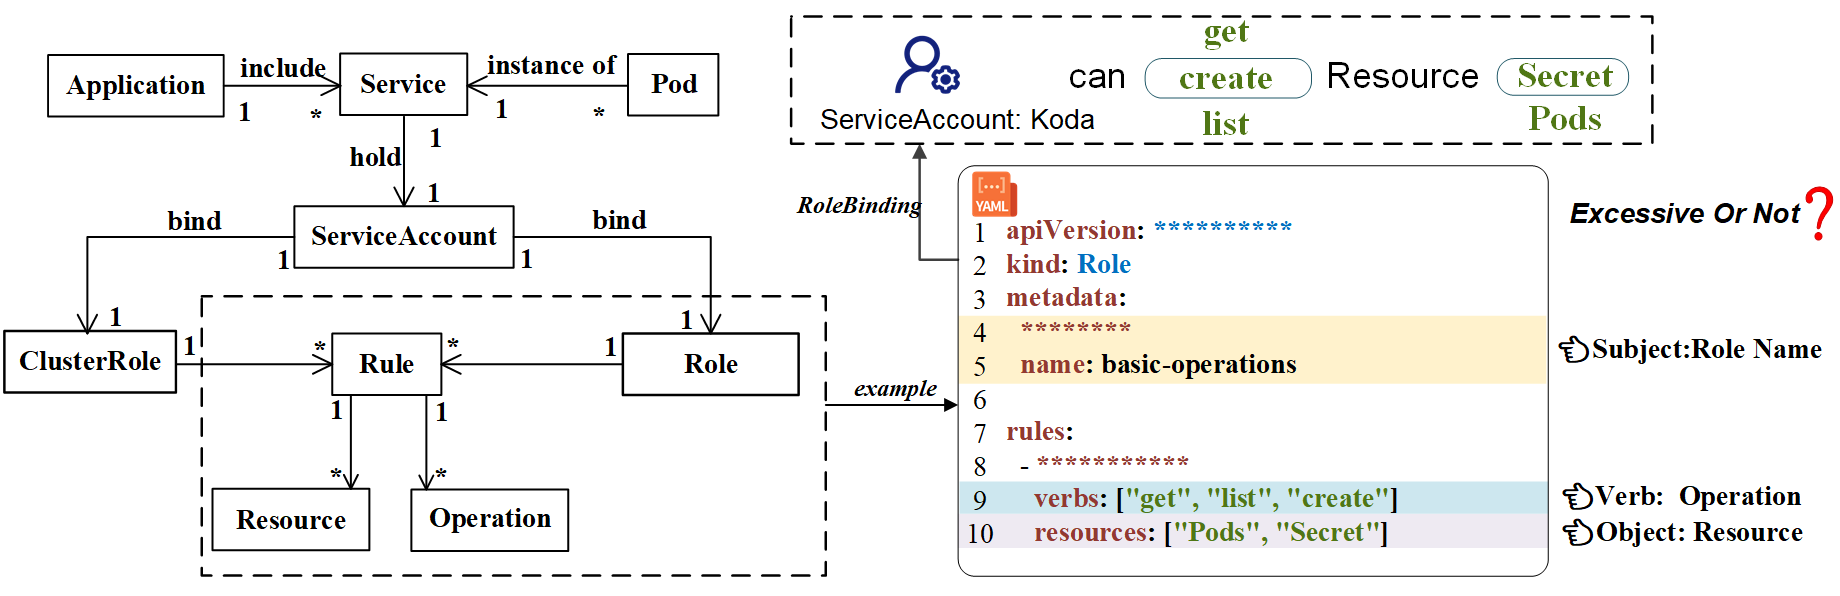
\includegraphics[width=0.95\linewidth]{pic/yaml.png}
    \caption{Permission metamodel and permission configuration instance}
    \label{fig:PM}
\end{figure*}

To overcome the aforementioned limitations, we propose a systematic permission-oriented risk detection approach called \kg. \kg conducts a step-by-step permission-oriented risk detection to safeguard the third-party applications. Specifically, during the pre-deployment phase, it first constructs a minimal permission set and then employs it to identify excessive permissions in given permission configurations. During the execution phase, it leverages a dynamic rule-based auditing technique to identify and intercept privilege escalation operations, and in the meanwhile monitors all messages transferred between $Pods$ and produces the alerting message in case sensitive resources are involved through the keyword matching. We further developed a supporting prototype called \kger and  conducted a series of experiments to evaluate the detection effectiveness and precision of \kg. The main contributions made in this study are as follows:

\begin{enumerate}
\item A systematic permission-oriented risk detection approach for third-party K8s applications called \kg is proposed, which targets the detection of excessive permissions at the pre-deployment phase, and privilege escalations and sensitive resources transmission at runtime.
\item A prototype called \kger is further developed to automate the proposed approach as much as possible.
\item Comprehensive experiments are conducted on a suite of open-source K8s applications to evaluate the  effectiveness of \kg in terms of detecting excessive permissions and privilege escalation and preventing from the sensitive resource linkage.
\end{enumerate}

The reminder of the paper is organized as follows. Section~\ref{sec:background} introduces the permission model of K8s and its potential threats. Section~\ref{sec:approach} presents our approach \kg and the implementation of supporting prototype \kger. Section~\ref{sec:ExperimentEvaluation} reports on the evaluation of the proposed approach. Section~\ref{sec:rw} discusses the related work. Finally, Section~\ref{sec:con} concludes the paper.

\section{Background} 
\label{sec:background}

This section introduces the basic concepts on the permission model of K8s and discusses the potential threats. 

\subsection{Permission Model}

K8s provides a practical service coordination paradigm and ensures the security of coordinated services (i.e., an application) through a permission model as depicted in the left part of Figure~\ref{fig:PM}. Specifically, an $Application$ consists of multiple $Services$ which are instanced as $Pods$ (work units). Each $Pod$ is assigned with a $ServiceAccount$. For a $ServiceAccount$, it can be bound with a $Role$ or $ClusterRole$. A $Rule$ specifies the allowed $Operations$ of a certain $Role$/$ClusterRole$ on some $Resources$. A $Resource$ is a persistent entity that describe the state, configuration, and services provided by K8s, including computational workloads (e.g., $Pod$, sensitive data storage (e.g., $Secret$) and declarative configuration entries (e.g., $ConfigMap$). Currently, there are a total of more than 50 types of $Resources$. 

K8s employs an extended Role-Based Access Control (RBAC) mechanism~\cite{ferraiolo1995role} to manage the access and manipulations of resources. An application must be assigned the corresponding permissions during the pre-deployment phase in order to access or manipulate resources within K8s at run-time. The right part of Figure~\ref{fig:PM} illustrates an example of permission configuration in K8s. In this case, the $ServiceAccount$ of  $Koda$ is bound with a $Role$ of $basic-operations$. Accordingly, this role is associated with a set of rules. One rule specifies that the $basic-operations$ role is allowed to perform $get$, $list$, and $create$ operations on $Pods$ and $Secret$ resources.

\subsection{Potential threats}
\label{ss:PotentialThreats}

\subsubsection{Excessive Permission}
\label{pt:ep}

When an third-party application is assigned with excessive permissions, K8s will be faced with various security risks. Consider the permission configuration illustrated in Figure~\ref{fig:PM}, the  permission of the $create$ operation on $Pods$, denoted as $PodCreation$, could be be risky. Assume that the $PodCreation$ permission is mistakenly assigned to a malicious application which holds the $Koda$ account. The application may make use of the $PodCreation$ permission to maliciously create an arbitrary number of $Pods$. Besides, the malicious $Pods$ could  be further used for security threats, such as data leakage, resource exhaustion, and DDoS attacks.

\subsubsection{Privilege Escalation}

Another potential threat source is privilege escalation~\cite{yang2023take}, which originates from excessive permissions. Again, consider the permission configuration illustrated in Figure~\ref{fig:PM}, the permission of the $get$ operation on $Secret$, denoted as $SecretGet$, could be used for privilege escalation. Assume that the $SecretGet$ permission is assigned to a malicious application which holds the $Koda$ account and the administrator keys are stored in the $Secret$ resource. In this context, the malicious application can obtain the keys and thus take over the management of worker nodes or even the whole cluster in K8s.

\subsubsection{Sensitive Resource Leakage}

Unmonitored messages transferred between $Pods$ could be the carrier of sensitive $Resources$, posing the potential threats to K8s. For instance, two applications are running on K8s with the $ServiceAccount$ of $Koda$ and $Tom$, respectively, as shown in Figure~\ref{fig:sil}. Assume $Pod-4$ needs to use the $Koda$ account to obtain the password for accessing database which are stored in the sensitive $Secret$ and the $Tom$ account has the permission for external communications. In this context, the password may be exposed outside the cluster along the message chain and thus the security of K8s is threaten.
%fig 2
\begin{figure}[!htb]
    \centering
    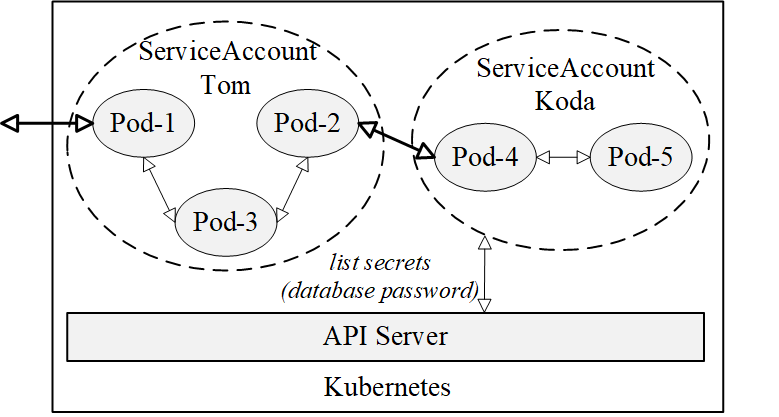
\includegraphics[width=8.5cm]{pic/sensive_pac.png} 
    \caption{An illustration of sensitive information leakage in K8s}
    \label{fig:sil}
\end{figure}

Although there exists some studies on risk assessment of K8s~\cite{k8smanifests2023,krane2024,kubiscan2024}, they have not well addressed the detection of the aforementioned threats. To detect excessive permissions and privilege escalation, existing techniques predominantly rely on static configuration analysis, without taking into account the dynamic orchestration nature of K8s~\cite{paloalto2024,k8smanifests2023,yang2023take}. Additionally, no work is reported on addressing K8s-specific sensitive $Resources$ leakage. 

%fig 3
\begin{figure*}[!tbh]
    \centering  
  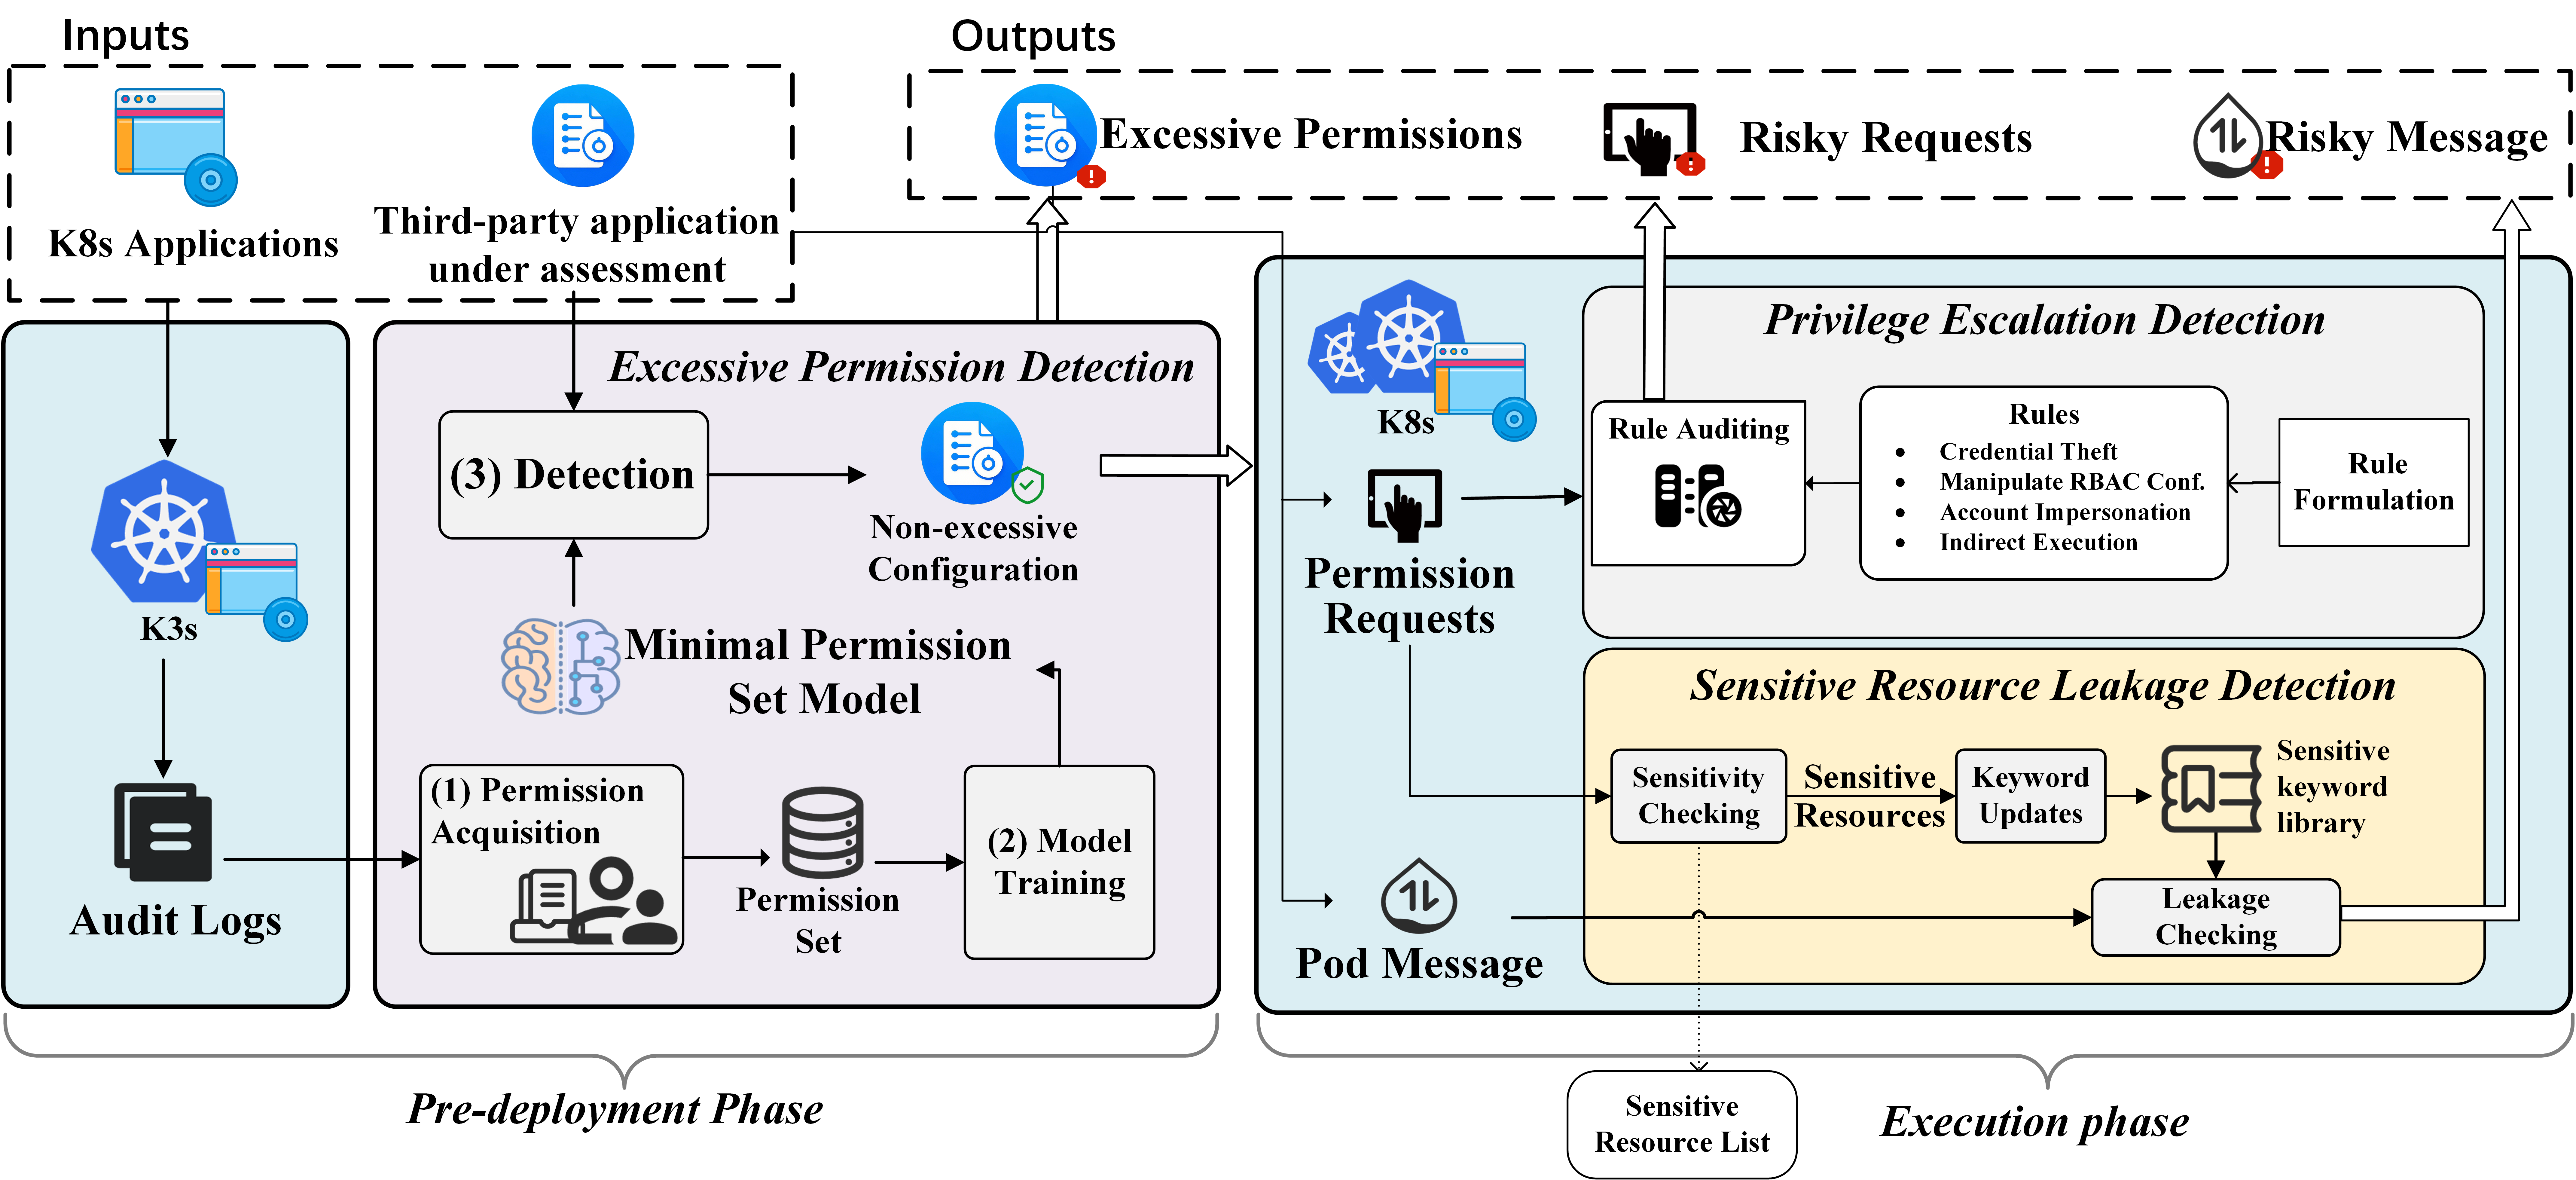
\includegraphics[width=0.9\linewidth]{pic/KGF.png} 
    \caption{Framework of \kg}
    \label{fig:KubeGuard}
\end{figure*}

\section{Approach} 
\label{sec:approach}

In this section, we first present the overview of our approach \kg and then discuss its key issues and prototype implementation.

\subsection{Overview} 
\label{sec:overview}

To address the limitations and the gap mentioned in Section~\ref{ss:PotentialThreats}, we propose a systematic permission-oriented risk detection approach called \kg. Figure~\ref{fig:KubeGuard} shows its framework. One can observe that \kg not only examines the existence of potential risks in the permission configurations during the pre-deployment phase, but also detects run-time privilege escalation and sensitive resource leakage during the execution phase. 
Specifically, \kg works as follows:

\begin{itemize} 
\item {\textit{During the pre-deployment phase}}, we first deploy third-party applications on a K3s~\cite{k3sdocs}, a lightweight K8s, and collect their audit logs for obtaining a part set of permissions, which, together with supplemental permissions, form a permission set. A minimal permission set model is obtain through a training process over the permission set. Based on the model, we examine whether excessive permissions exist in the permission configuration of the given third-party application under assessment. 

\item{\textit{During the execution phase}}, we migrate the third-party application that passes the \textit{Excessive Permission Detection} to a production-level K8s cluster after eliminating excessive permissions. \kg dynamically intercepts all permission requests and applies a rule-based auditing process to detect privilege escalation risks. In the meanwhile, the messages transferred between $Pods$ are monitored to alert potential risks of sensitive resource leakage. 
\end{itemize}

\subsection{Excessive Permission Detection} 
\label{sec:epd}

Given a permission configuration of an third-party application, one feasible way for judging whether excessive permissions exist is to compare the configuration against a \textit{ground truth permission set}, which is hard or even impossible to obtain in practice because heavy manual efforts are required to analyze the permission specification of K8s. Inspired by the principle of least privilege (POLP)~\cite{saltzer1975protection} that every privileged user of the system should operate using the least amount of privilege necessary to complete the job, we propose the concept of the \textit{Minimal Permission Set} for K8s applications. Let $R$ be the set of all $Resources$ in K8s, $SA$ be the set of a third-party application $ServiceAccount$\footnote{Note that an application may have multiple $ServiceAccounts$ with respect to different $Pods$} and $Verb$ is all permitted $Operations$. The set of all possible permissions for a third-party applications is denoted as $U_{all} = SA \times Verb \times R$. Now, $U_{all}$ can be divided into two parts: the minimal permission set $U_m$ and the excessive permission set $U_e$. $U_m$ is the least one among the set of permission sets that enables an application to fulfill its intended functions. Obviously, it can be inferred that \(U_m = U_{all} - U_e\). The key to excessive permission detection is to determine a binary excessive permission classifier $f$ such that:

\begin{equation}
\label{equ:classfierf}
f(PT) = \left\{
    \begin{aligned}
        &1, && \text{if } PT \in U_m, \\
        &0, && \text{if } PT \in U_e.
    \end{aligned}
\right.
\end{equation}
Alternatively, we build a minimum permission set model based on the permission request records in the audit logs of K8s and inspect the built model before the detection of excessive permissions.

%which is the set of permissions required for all third-party applications to fulfill their intended business functions.The objective of this part is to accurately identify $U_e$ from $U_c$.

% These execution patterns dictate that the minimum permission set $U_m$ follows a specific distribution in the feature space of permissions. The historical set of permissions executed in the cluster is defined as the historical permission set. We can infer:
%The permissions required by an application are typically closely related to its business requirements. 
%Permission  for third-party application $ServiceAccount$ are generally defined by the developers of those applications. Adhering to the principle of least privilege and standardizing these configurations necessitates the detection of excessive permissions to eliminate excess access rights. 

%We have constructed a binary classification model like $f$ in equation~\ref{equ:classfier} that utilizes the BERT~\cite{devlin2018bert} pre-trained model to mine the access patterns of third-party application permissions in audit logs. This provides users with review recommendations for excessive permission risks. This approach not only integrates historical permission accesses into the minimal privilege set but also marks semantically similar permissions in the audit logs as available permissions. 

\subsubsection{Permission Acquisition}
\label{sec:permission_acquisition}

The permission requirement of an application is closely related to its functionalities and is reflected as the permission request in K8s during the execution. For example, Prometheus frequently requires $list$ permissions for Pods, Nodes, and Services, while CI/CD tools require $create$ and $update$ permissions for deploying and updating the applications. Fortunately, the audit logs recording permission requests could be used for identifying the permission usage of an application~\cite{wei2024log}. 

%Namely, by exploiting the information of \(U_h\) and \(U_{all} - U_c\), a learning model is leveraged to bridge the uncertainty of \(U_c - U_h\), which includes three steps.

A high-quality permission benchmark set is crucial for training the permission detection model in order to achieve good precision. Unfortunately, such a set for this purpose is still absent. Alternatively, we construct this benchmark as follows (refer to the left part of Figure~\ref{fig:PRel}): 1) We first run a set of diverse applications on K3s and collect the historical permissions (denoted as $U_h$) from their audit logs~\footnote{https://kubernetes.io/docs/tasks/debug/debug-cluster/audit/}; 2) The inspected historical permissions ($U_{h'}$), together with supplemental correct permissions ($U_{supp}$) to cover all possible permissions $U_{all}$, form a positive sample set; 3) Some noisy permissions $U_{noisy}$ obtained through the mutation of $U_{h'}$ form a negative sample set; 4) Finally, a comprehensive benchmark is constructed by composing the both sets.    

%Obtaining the binary excessive permission classifier $f$ is an  objective, but we cannot directly obtain the complete \(U_m\) or \(U_e\). However, we can obtain the audit logs recording permission requests by running the applications. The historical set of permissions requests in the cluster is defined as the historical permission set $U_h \subseteq U_m$. The set of permissions configured for third-party applications in K8s is denoted as $U_c$. The relationships between $U_{all}$, $U_c$, $U_m$, and $U_h$ are shown in Figures~\ref{fig:aus}. 

\begin{figure}[!htb]
    \centering
    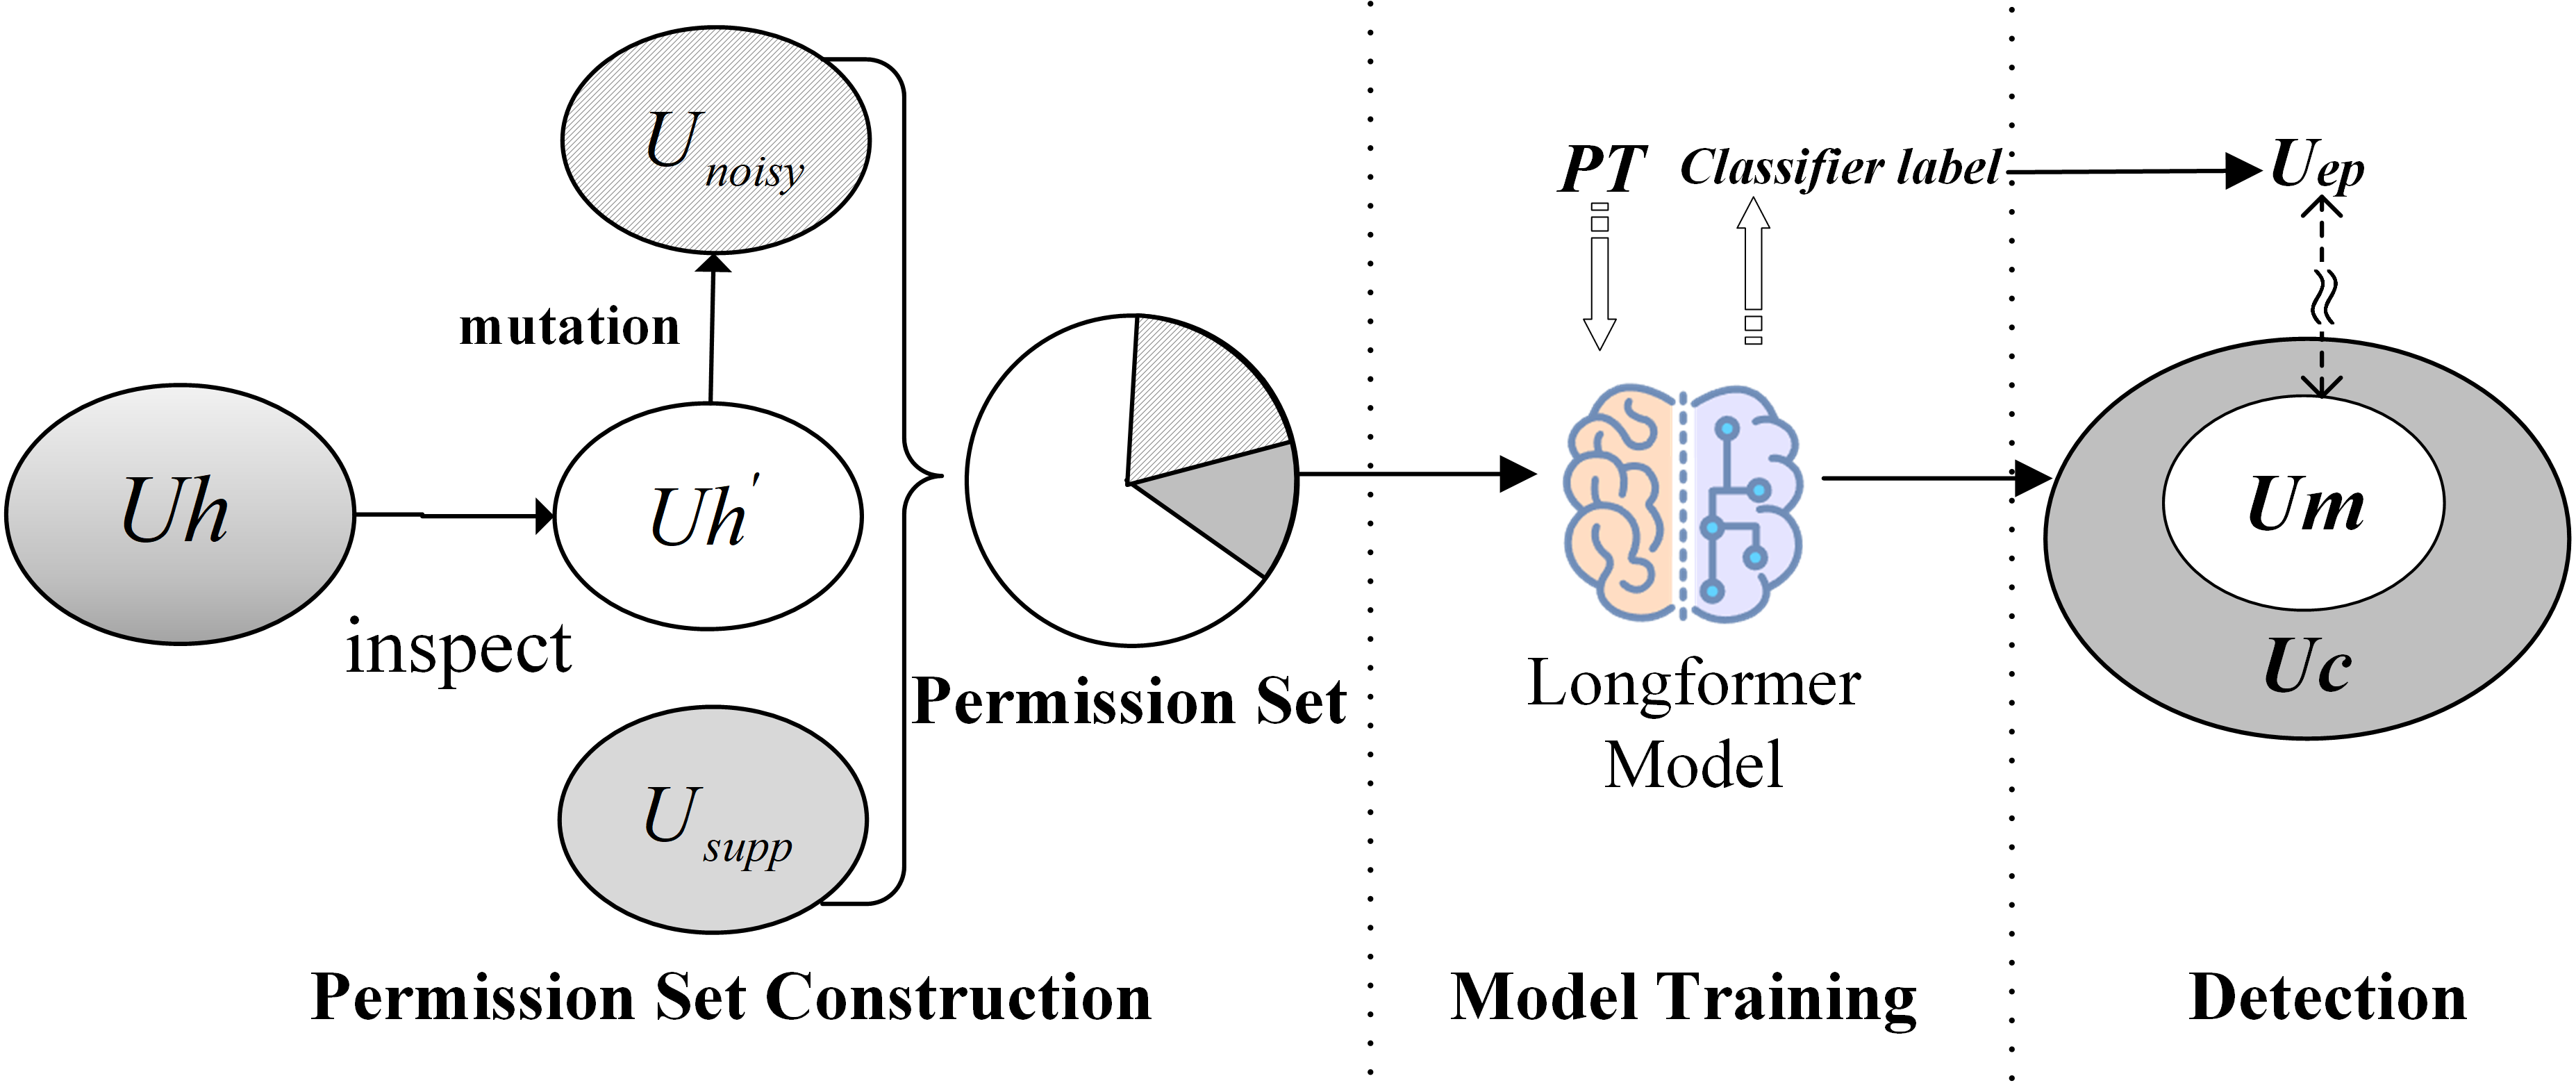
\includegraphics[width=1\linewidth]{pic/permision_set_con.png} 
    \caption{Minimal-set-based excessive permission detection}
    \label{fig:PRel}
\end{figure}

%Based on \(U_h\) and \(U_c\), we obtain an incomplete classifier.
%\begin{equation}
%\label{equ:classfierg}
%f'(PT) = \left\{
%    \begin{aligned}
%        &1, && \text{if } PT \in U_h \\
%        &0, && \text{if } PT \in U_{all} - U_c \\
%        &uncertain, &&  \text{if } PT \in U_c - U_h
%    \end{aligned}
%\right.
%\end{equation}

%The purpose of this step is to construct a permission set for model training. First, parse the permission access requests recorded in K8s audit logs\footnote{https://kubernetes.io/docs/tasks/debug/debug-cluster/audit/} to obtain \(U_h\). Then, the Cartesian product of $ServiceAccount$, $Resources$, and  \textit{Operations} from the K8s context is calculated to form $U_{all}$. And based on the RBAC configuration, valid permissions in $U_{all}$ are identified and included in $U_c$. Under manual review, we label $U_h$ as non-excessive permissions (positive examples) and $U_{all} - U_c$ as excessive permissions (negative examples), thus constructing a permission set for training the minimum permission set model. 

\subsubsection{Model Training}

Permission configurations consisting of a large number of permissions could be very complex in some situations. As discussed above, a permission in the original permission model involves ($ServiceAccount$, $Role/ClusterRole$, $Operation$, $Resource$), and other information such as $namespace$ and $apiGroups$. To ease the model training, we simplify them as a \textit{permission triple}: $PT = \langle ServiceAccount, Operation, Resource \rangle$, with which a permission configuration is represented as a set of $subject-verb-object$ entries. Each entry specifies the specific $Operation$ ($verb$) of a $ServiceAccount$ ($subject$) on a given $Resource$ ($object$). Table~\ref{tab:features} illustrates a simplified permission configuration with a total of eleven features. These features are concatenated as a vector with the separator token $[SPE]$, allowing for distinguishing different dimensions and carrying semantic information.

%Additionally, the omission of $namespace$ and $apiGroups$ will not affect the subsequent detection of excessive permissions.
%\begin{definition}[\textit{Permission Triple}] %\label{def:permission} 
%    \begin{equation} 
%        \begin{split} PT = \langle ServiceAccount, %Operation, Resource \rangle\end{split} 
%    \end{equation}
%\end{definition}
%For each permission, we concatenate three dimensions with a total of 11 permission details (as shown in Table~\ref{tab:features}) using the separator token $[SPE]$. This optimization enables the machine learning model to distinguish between different dimensions of permission data entry, and  enriches the semantic information. 

\begin{table}[!ht]
    \centering
    \caption{Illustration of Permission Features and Dimensions}
    \label{tab:features}
    \renewcommand{\arraystretch}{1.2} % 行距
    \setlength{\tabcolsep}{0.5mm} % 列间距
    \begin{tabular}{p{2cm}p{2cm}p{4cm}}
    \toprule
    \textbf{Category} & \textbf{Feature} & \textbf{Example} \\ 
    \hline
    \multirow{4}{*}{\textit{ServiceAccount}} & Name & \texttt{prometheus-operator} \\ 
                                    & Namespace & \texttt{monitoring} \\ 
                                    & Labels & \texttt{app.name:
                                    "prometheus-operator"} \\ 
                                    & Annotations & \texttt{\{\}} \\ 
    \hline
    \multirow{6}{*}{$Resource$}       & Namespace & \texttt{monitoring} \\ 
                                    & Group & \texttt{apps} \\ 
                                    & Kind & \texttt{Deployment} \\ 
                                    & Name & \texttt{kube-state-metrics} \\ 
                                    & Labels & \texttt{app.name: "kube-state-metrics"} \\ 
                                    & Annotations & \texttt{default-container: "kube-state-metrics"} \\ 
    \hline
    \textit{Operation} & Verb & \texttt{get} \\ 
    \bottomrule
    \end{tabular}
\end{table}

%The purpose of this step is to construct a permission set for model training. First, parse the permission access requests recorded in K8s audit logs\footnote{https://kubernetes.io/docs/tasks/debug/debug-cluster/audit/} to obtain \(U_h\). Then, the Cartesian product of $ServiceAccount$, $Resources$, and \textit{Operations} from the K8s context is calculated to form $U_{all}$. And based on the RBAC configuration, valid permissions in $U_{all}$ are identified and included in $U_c$. Under manual review, we label $U_h$ as non-excessive permissions (positive examples) and $U_{all} - U_c$ as excessive permissions (negative examples), thus constructing a permission set for training the minimum permission set model.

We design the minimal permission set model based on $longformer$~\cite{beltagy2020longformer}, which is a pre-train BERT-like model~\cite{devlin2018bert}. Figure~\ref{fig:bert} shows the model structure and data flows of $longformer$. Specifically, a 1024 token window is set to handle longer text information. In most situations, a vector of features in Table~\ref{tab:features} exceeds the token length limit (512 tokens) of standard BERT models. After training with the benchmark discussed in Section~\ref{sec:permission_acquisition}, we have built a minimal permission set model that accepts a permission of $PT$ and outputs a classifier label (Boolean variable), indicating whether the permission is excessive or not, as shown in the middle part of Figure~\ref{fig:PRel}. 

\begin{figure}[ht]
    \centering
   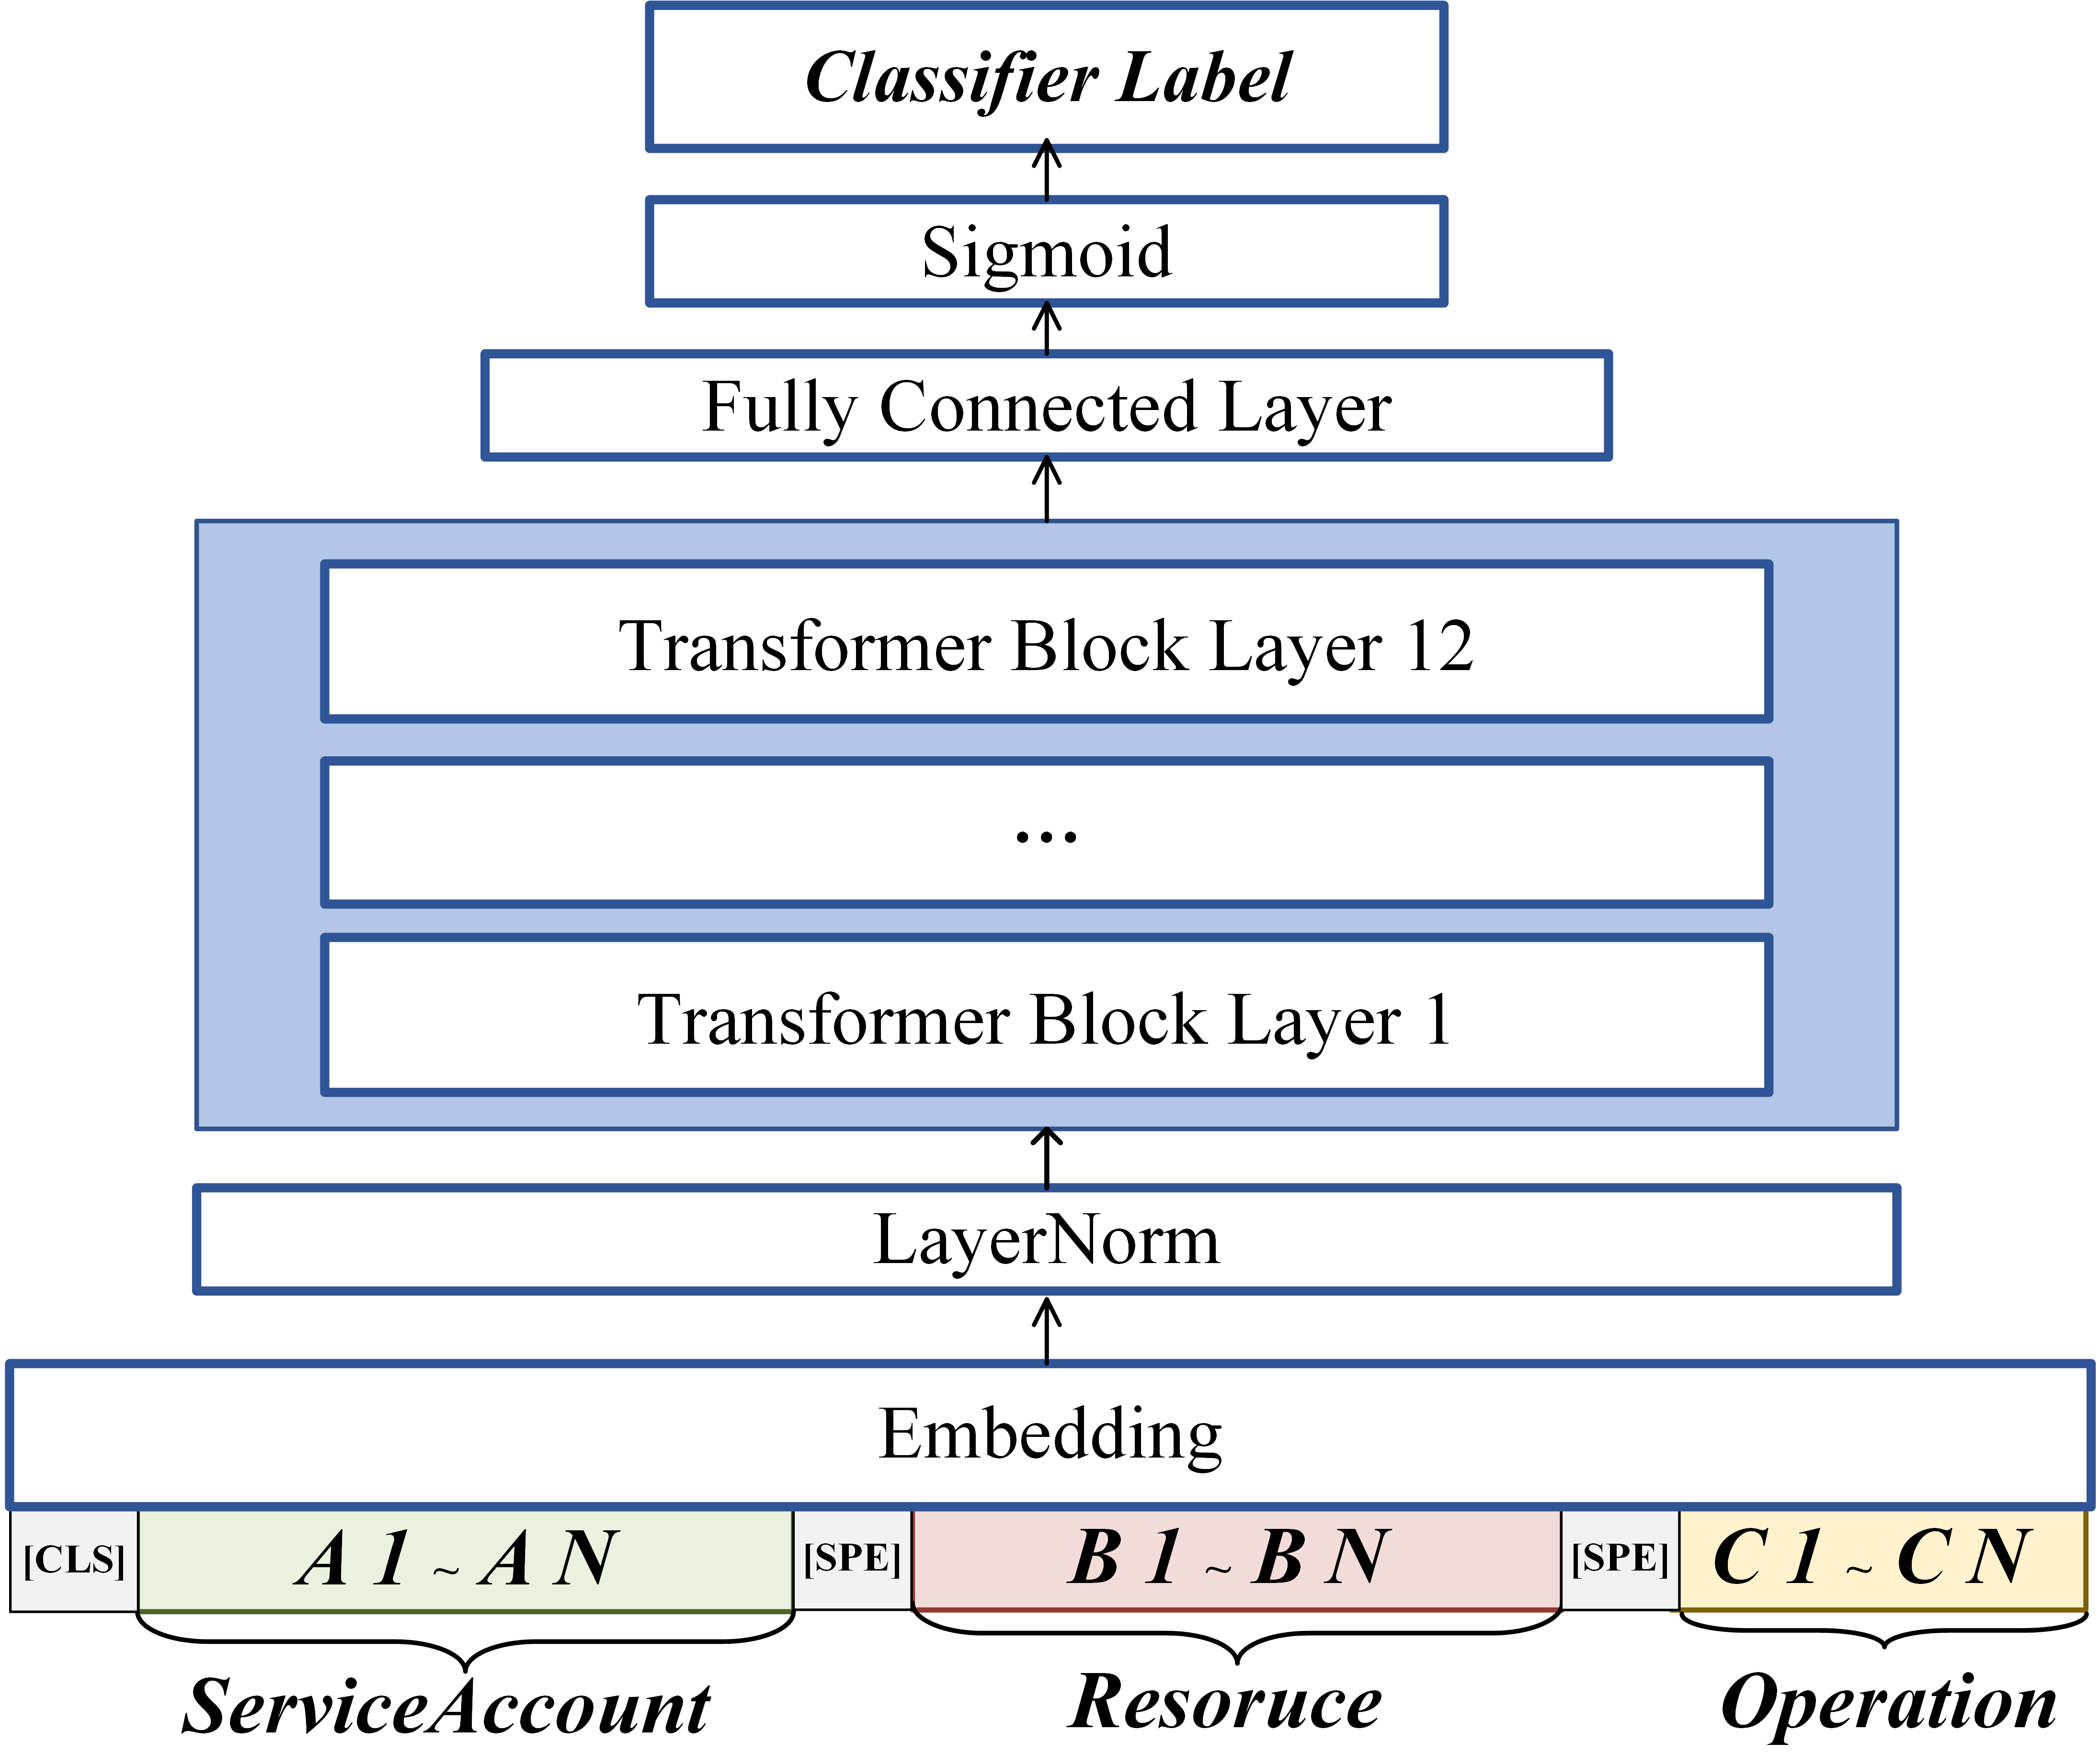
\includegraphics[width=0.85\linewidth]{pic/BERT.png}
    \caption{Network model architecture and data flows of longformer}
    \label{fig:bert}
\end{figure}

\subsubsection{Detection}

 %The YAML-formatted permission configuration has to be transformed into the permission triples $PT$ and subsequently fed into the minimal permission set model. Thus, we obtained a non-excessive permission configuration and the excessive permissions from the original configuration.

Given a YAML-formatted permission configuration $U_c$ of the third-party application under assessment, we first extract all permission entries. For each permission inside of $U_c$, it is first transformed into a $PT$ and then fed into the $longformer$ model. According to the returned classifier label, we can determine whether the current permission is excessive or not. Only those non-excessive permissions are included in an expected permission set $U_{ep}$, which is used as an approximate minimal permission set $U_m$, as shown in the right part of Figure~\ref{fig:PRel}. Finally, the detected excessive permissions are  $U_e = U_{c} - U_m$.

%the relationship between different set of permission is shown in Figure~\ref{fig:PRel}. Note that in practice, historical permissions, minimum permissions, permission configuration, exhaustive permissions....  .... inspect historical permission and supplement extra permissions are necessary.... why.... how to do.... Algorithm....

\subsection{Privilege Escalation Detection} 
\label{sec:escalation}

Unlike excessive permissions that can be detected through static analysis of permission configurations during the pre-deployment phase, precision detection of privilege escalation risks can only be achieved at runtime. Specifically, \kg turns to permission requests for this purpose. In the context of K8s, to perform an operation on a specific $Resource$, a Pod $sourcePod$ associated with an IP address $IP$ and an account $ServiceAccount$ has to send a \textit{permission request} $PR = (sourcePod, IP, ServiceAccount, Operation, Resource)
$. According to the official K8s documentation~\cite{kubernetes2024} and related studies~\cite{yang2023take,paloalto2024}, we summarize four types of privilege escalation, as shown in Table~\ref{tab:PEDetectionRules}.

\begin{table*}[!ht]
    \centering
    \caption{Various privilege escalation and their detection rules}
    \label{tab:PEDetectionRules} 
    \renewcommand{\arraystretch}{1.1}
    \setlength{\tabcolsep}{3mm}
    \begin{tabular}{m{3cm}m{4cm}>{\raggedright\arraybackslash}p{9.5cm}}
    \toprule
    \textbf{Type} & \textbf{Mechanism} & \textbf{Detection Rule}\\ 
    \midrule
    % CT
    \multirow[t]{3}{2cm}{Credential Theft  (CT)} 
    & \texttt{- Secret Access} 
    & \multirow{3}{9cm}{
        \vspace{-2.9ex} 
        \begin{equation*}
            PR_{CT} = \left\{ PR \, \middle| \, 
            \begin{aligned}
                & PR.IP \neq RP.sourcePod.IP \land \\ 
                &  \, PR.ServiceAccount \neq PR.sourcePod.ServiceAccount
            \end{aligned}
            \right\}\quad\quad\quad 
        \end{equation*}
        \vspace{3ex} 
        } \\
    & \texttt{- Pod Exec} \\
    & \texttt{- Container Escape} \\
    \midrule
    
    \multirow[t]{2}{2.7cm}{Account Impersonation  (AI)} \vspace{0.7ex}
    & \texttt{- ServiceAccount Impersonation} 
    & \vspace{-5.8ex} \begin{equation*}
        PR_{AI} = \{ PR \mid (PR.ServiceAccount, PR.Operation, PR.Resource) \notin U_{acc} \}\quad
    \end{equation*}
    \vspace{-2.8ex}
     \\ 
    \midrule

    % RBAC manipulation
    \multirow[t]{3}{3cm}{RBAC Manipulation \\ (RM)\qquad\qquad\qquad} 
    & \texttt{- Role Modification}
    & \multirow{3}{9cm}{
        \vspace{-3ex}
    \begin{equation*} 
        PR_{RM} = \left\{ PR \, \middle| \, 
            \begin{aligned}
                & PR.Operation \in \{ \text{create, patch, update} \} \\
                & \land \, PR.Resource \in \{ \text{Role}, \text{ClusterRole}, \\& \text{RoleBinding}, \text{ClusterRoleBinding} \}
            \end{aligned}
        \right\} \qquad\qquad\qquad
    \end{equation*}
    } \\
    & \texttt{- RoleBinding Modification } \\
    & \\
    \midrule

    % indirect execution
    \multirow[t]{2}{2.5cm}{Indirect Execution \quad  (IE) }
    & \texttt{- Workload Modification} 
    & \multirow{2}{9cm}{
        \vspace{-4.1ex}
       \begin{equation*}
        \label{equ:ie}
        PR_{IE} = \left\{PR \, \middle| \, 
        \begin{aligned}
            & (PR.Resource \in WL \land Pr.Operation \in \{ \text{create} \\
            & \quad \text{patch, update} \}) \vee PR \in (*,*,*, \text{exec}, \text{Pod})
        \end{aligned}
        \right\} \quad\quad\quad\quad
    \end{equation*}
        } \\
    & \texttt{-  Pod Exec} \\
    \bottomrule
    \end{tabular}
\end{table*}

For each type of privilege escalation, we further elaborate its implementation mechanism, formulate its detection rule based on which all permission requests are audited individually. 

\subsubsection{Credential Theft (CT)}
K8s authenticates service accounts using JWT. If a $Pod$ illegally obtains the credentials of other service accounts, it can access all the permissions associated with them. CT can be implemented in the following ways:
\begin{itemize}
  \item \textit{Secret Access:} Credentials of a $ServiceAccount$ are often stored in $Secret$ $Resource$. An attacker could obtain all credentials of $ServiceAccount$ within the namespace by accessing the Secret.
  \item \textit{Pod Exec:} Credentials of the bound $ServiceAccount$ are mounted in the Pod's file-system (default path:$/var/run/secrets/kubernetes.io/serviceaccount$). An attacker could use the $exec$ Request to access and steal the credentials.
  \item \textit{Container Escape:} An attacker could exploit vulnerabilities or misconfigurations in the container to gain the access to the host or other containers through directory mounting, and access sensitive resources and credentials.
\end{itemize}

Based on the implementation mechanisms, we formulate the detection rule of credential theft $PR_{CT}$: The $ServiceAccount$ and $IP$ associated with the $sourcePod$ are compared with those credentials involved in the $PR$. Any mismatch indicates a potential credential theft. This detection rule applies to all attack implementations discussed above.

\subsubsection{Account Impersonation (AI)}
K8s supports impersonation permission function since version 1.4, allowing one $ServiceAccount$ to perform permission request as another one. This is mainly used for debugging permission configurations but may be abused by malicious third-party applications. Account impersonation occurs when an $PR$ is performed under an impersonated account with permissions outside the scope of the original $ServiceAccount$. 

The detection rule of account impersonation $PR_{AI}$ is as follows: For each $PR$, a secondary compliance review is conducted for the $ServiceAccount$ involved in $PR$, where $U_{acc}$ represents the set of permissions for the actual $ServiceAccount$. 

\subsubsection{RBAC Modification (RM)}
K8s treats permission configurations as a kind of $Resource$. If a $Pod$ has permissions to modify such a permission configuration resource, the privilege escalation risk exists because it can modify the related permission configuration. $RM$ can be implemented as follows:
\begin{itemize}
  \item \textit{Role Modification:} The $Role$ or $ClusterRole$ resource are allowed to modify through the \textit{create/patch/update} operations.  
  \item \textit{RoleBinding Modification:} The $RoleBinding$ or $ClusterRoleBinding$ resources are allowed to modify through the $create/patch/update$ operations.
\end{itemize}

The detection rule of RBAC modification $PR_{RM}$ is as follows: For a given $PR$, we examine whether there exists a $create$, $patch$ or $update$ on $Role$, $ClusterRole$, $RoleBinding$, or $ClusterRoleBinding$ involved in the permission configuration. 

\subsubsection{Indirect Execution (IE)}
A group of $Pod$, $ReplicaSet$, $Deployment$, $StatefulSet$, $DaemonSet$, $Job$, and $CronJob$ is workload-related $Resources$ in K8s, denoted as $WL$, which are used for application execution and management. $ServiceAccount$ with $WL$ permissions can indirectly execute unexpected operations by creating or controlling workload related $Resources$. 
\begin{itemize}
  \item \textit{Workload Modification:}  Permission requests that modify $WL$ could create Pods using any other $ServiceAccounts$, which may further perform unexpected permission requests.
  \item \textit{Pod Exec:} The $exec$ Operation on a $Pod$ allow a $SeriviceAccount$ to run commands and scripts arbitrarily, which may control the $Pod$ of other applications to perform unexpected permission requests.
\end{itemize}

The detection rule of indirect execution  $PR_{IE}$ is as follows: For each $PR$, we examine whether there are any modification operations on $WL$ and whether there exist $exec$ operation on other Pods.

% Permission Request rule-based auditing leverages the authentication webhook of the K8s management-stage services, which can capture detailed information of each permission request. Based on the four rules, we conduct a sequential rule-based audit to detect permission requests with privilege escalation risks.

\subsection{Sensitive Resource Leakage Detection} 
\label{sec:leakage}

In the context of K8s, a third-party application is deployed on a cluster of $Pods$, sensitive resources can be leaked only through the messages transferred between $Pods$ with the approved permission request on the resource. Accordingly, \kg detects possible sensitive resource leakage through monitoring transferred messages between Pods and examines whether sensitive resources are carried. 

% fig 6
 \begin{figure}[!htb]
    \centering
    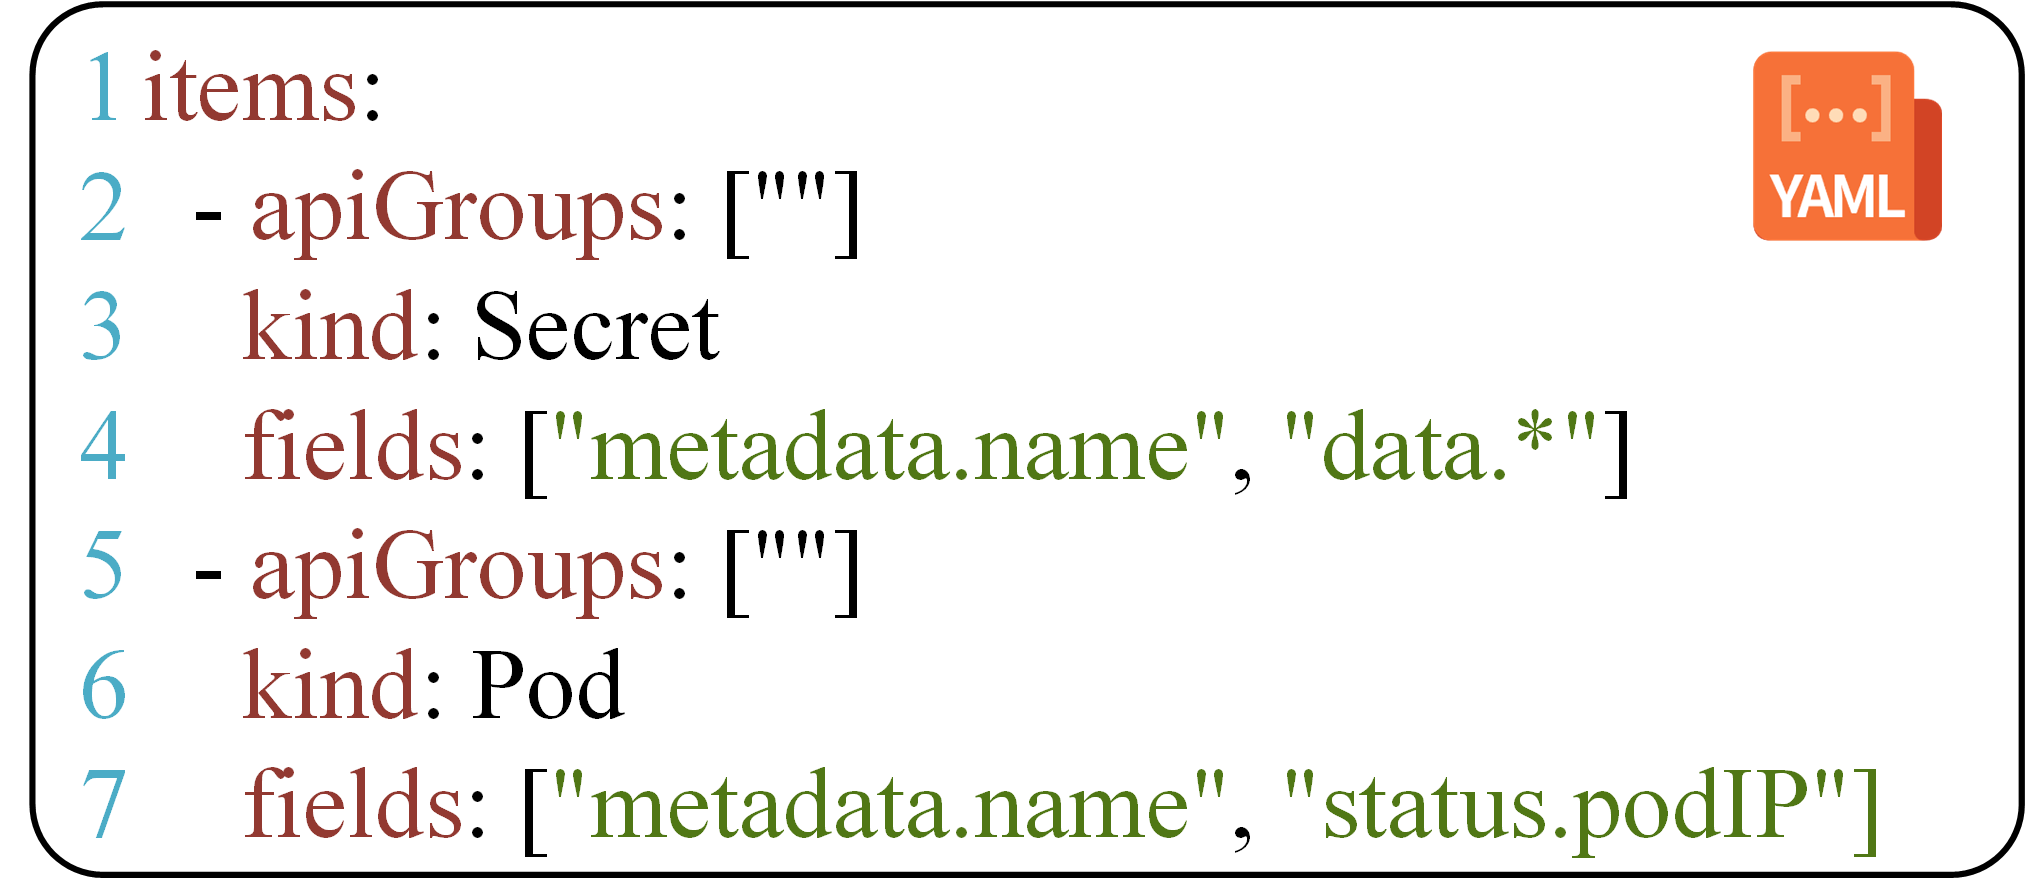
\includegraphics[width=0.7\linewidth]{pic/yaml2.png}
    \caption{An example of sensitive resource list $SRL$}
    \label{fig:sen_conf}
\end{figure}

\subsubsection{Sensitivity Checking} Sensitive resources could be either system credentials, such as system accounts and passwords, or variables of an application carrying sensitive information. To support a configurable sensitive resource leakage, \kg uses a Sensitive Resource List ($SRL$) to specify the desired sensitive resources. Specifically, $SRL = \{item_1, item_2, \ldots, item_n\}$, where each item is a triplet: $item = (apiGroups, type, keys)$. Figure~\ref{fig:sen_conf} illustrates an example of $SRL$. Here, $apiGroup$ is a namespace for identifying resources; $type$ is used to specify the type of resources; $keys$ are a set of strings to specify the keywords of sensitive resources. In this example, $Secret$ and $Pod$ are sensitive resources, the $metadata.name$ and any strings starting with $data.$ are keys of $Secret$, and the $metadata.name$ and $status.podIP$ are keys of $Pod$. With the $SRL$, K8s administrators can specify their desirable sensitive resources, and each permission request will be checked whether the specified resources are involved. 


\subsubsection{Keyword updates}
Once a permission request involving sensitive resources is approved, the detailed information will be responded. The involved resources may be accessed intermediately or continuously. In this situation, it is necessary to maintain a keyword library on the information of involved sensitive resources to support the subsequent leakage checking.     

The sensitive keyword library contains a set of  mappings, i.e., $SKL = \{(SA, KL)\}$, where $SA$ is a $ServiceAccount$ and $KL$ is a list of keywords for sensitive resources permitted to $SA$. The process of keyword updates in the $SKL$ described as Algorithm~\ref{alg:sensitive_lib_construct}. For each $PR$, its retrieved resources is checked against $SRL$, and if the resource belongs to $SRL$, associated $ServiceAccount$ of $PR$ and $item$ of the resource are appended to $SKL$.

% algorithm 1
\begin{algorithm}[!hbt]
\caption{Keyword updates in the sensitive keyword library}
\label{alg:sensitive_lib_construct}
\begin{algorithmic}[1]
\Require{Permission Request $PR$, 
Sensitive Keyword Library ${SKL}$}
\Ensure{${SKL}$}
%\Function{updateKeywordsLibrary}{$PR$}
          \State $resource \gets \Call{GetResource}{PR}$
        \If{${resource} \in SRL$} 
            \State $SA \gets \Call{GetAccount} {PR}$ 
            \State $KL \gets \Call{ExtractSensitiveInfo}{resource}$
            \State ${entry} \gets (SA, KL) $ 
            \State ${SKL} \gets {SKL} \cup \{entry\} $
        \EndIf
    \State \Return ${SKL}$
%\EndFunction
\end{algorithmic}
\end{algorithm}

\subsubsection{Leakage Checking}
Based on the sensitive keyword library $SKL$, we can detect potential leakages through monitoring the messages transferred between Pods. These messages can obtained through parsing the packets between Pods. A packet is a quadruple, $packet = (srcIP, dstIP, request, response)$, where $srcIP$ and $dstIP$ are the IP addresses of the sender Pod and receiver Pod, respectively, $request$ and $response$ are the messages sent and received by $Pods$, respectively.

Algorithm~\ref{alg:sen_det} describes the detailed leakage checking process. Specifically, given a packet $Pk$, it first determines whether the $Pk$ is transferred between the $ServiceAccount$ of $srcAcc$ and $dstAcc$, which can be obtained through analyzing $srcIP$ and $dstIP$. If the two $ServiceAccounts$ not the same, $request$ and $response$ are checked against $SKL$ to whether any sensitive keywords are involved. A success match indicates a sensitive resource leakage risk.

%algorithm 2
\begin{algorithm}[!htb]
\caption{Leakage Checking}
\label{alg:sen_det}
\begin{algorithmic}[1]
\Require{Packet $PK$, Sensitive Keyword Library $SKL$}
\Ensure{Boolean flag indicating leakage risk}
    \State $risky \gets \text{False}$
    \State $srcAcc \gets \Call{GetServiceAccount}{PK.srcIP}$
    \State $dstAcc \gets \Call{GetServiceAccount}{PK.dstIP}$
    \If{$srcAcc \neq dstAcc$}
        \If{($srcAcc$, $PK.request$) $\in SKL$ $\vee\quad\quad\quad\quad\quad$ ($dstAcc$, $PK.response$) $\in SKL$}
            \State $risky \gets \text{True}$
        \EndIf
    \EndIf
    \State \Return $risky$  
%\EndFunction
\end{algorithmic}
\end{algorithm}
\vspace{-6pt}

\subsection{Prototype Implementation} 
\label{sec:impl}

We have developed a supporting tool called \kger, whose source code can be accessed through the website  \url{https://github.com/Ivanbeethoven/KubeGuarder}. \kger supports \kg in the following ways:
\begin{itemize}
  \item \textit{For excessive permission detection}, a component is developed for parsing K8s audit logs and adding negative samples randomly in order to obtain permission set as discussed in Section~\ref{sec:permission_acquisition}; The minimal permission set model is implemented based on Hugging Face~({\url{https://huggingface.co/}}) and PyTorch~({\url{https://pytorch.org/}}). The former provides an open-source implementation of $longformer$, while the latter is used for model training. %according to the token window parameters. 
  
  \item \textit{For privilege escalation detection,} a component is developed for run-time interception and auditing of permission requests via the K8s $Webhook$ (\url{https://kubernetes.io/docs/reference/access-authn-authz/extensible-admission-controllers/}), which is an extensible admission control mechanism for K8s; a component is implemented in Java for rule auditing.

  \item \textit{For sensitive resource leakage detection,} a component is developed to support the $SKL$ updates via the K8s $Webhook$; The interception of messages transferred between Pods is implemented based on \textit{Kubeshark}, which is a K8s-native traffic monitoring tool; Both Algorithms discussed in Section~\ref{sec:leakage} are implemented in Java.
\end{itemize}

\section{Experimental Evaluation} 
\label{sec:ExperimentEvaluation}

We conduct a series of experiments\footnote{The experimental raw data are available on the website \url{https://github.com/Ivanbeethoven/KubeGuarder/tree/master/evaluation} } to evaluate the effectiveness of \kg. 

\subsection{Research Questions}
\label{ss:RQ}

Through the experiments, we aim to answer the following research questions:

\begin{itemize}
\item \textit{RQ1:} How effective is \kg in detecting excessive permissions? and how does the model training influence the detection effectiveness?

We evaluate the accuracy, recall, and F1-score of \kg and baselines for a suit of subject applications. An ablation study is conducted to further assess the contributions of model training by comparing the precision of \kg and \textit{\kg w/o ML} (i.e., bypassing the model training). 

\item \textit{RQ2:} How effective is \kg in detecting privilege escalation? 

We simulate twenty privilege escalation scenarios covering all cases discussed in Table~\ref{tab:PEDetectionRules} and report the detection effectiveness of \kg.

\item \textit{RQ3:} How effective is \kg in detecting sensitive resource leakage?

We simulate around 1,600 leakage scenarios involving six types of sensitive resources and report the detection effectiveness of \kg.

\end{itemize}

\subsection{Subjects Applications}
We collected a suite of diverse open-source third-party K8s applications from the website (i.e., \url{https://artifacthub.io/}) for excessive permission evaluation, as summarized in Table~\ref{tab:3rd-app}, including the name, category, the size in thousands of lines of code, and the number of $ServiceAccount$ of applications.
Since there is not third-party application set available for the evaluation of privilege escalation and sensitive resource leakage, we employed an open-source K8s project available on the website of \url{ https://github.com/ewolff/microservice} to simulate a large number of privilege escalation and sensitive resource leakage scenarios for the evaluation.

%table III
\begin{table}[!htb]
\centering
\caption{A summary of third-party applications for excessive permission detection}
\begin{tabular}{llll}
\hline
\textbf{Name} & \textbf{Category} &\textbf{KLOC} &\textbf{\#Account}\\
\hline
GitLab & DevOps  & 1788.1& 7\\
Istio & Service Mesh & 496.4 & 5 \\ 
ArgoCD & DevOps & 359.5 & 5\\ 
Prometheus & Monitoring Tool& 252.9 & 5 \\ 
Cert-Manager & Management&  161.1 & 3\\ 
MetalLB & Load Balancer & 53.4 & 2  \\ 
Jenkins & DevOps&  319.6 & 1\\ 
Dashboard &  Management &  63.8 & 1 \\
Ingress-NGINX & Load Balancer & 75.0 & 1 \\ 
Kubeshark & Monitoring Tool & 6.0 & 1 \\
\hline 
\end{tabular}
\label{tab:3rd-app}
\end{table}
\vspace{-6pt}

\subsection{Experimental Settings} 
The experiments were designed as follows:
(1) For the excessive permission detection, we collected a total of 167,203 permission audit logs to construct \textit{the permission set} as discussed in Section~\ref{sec:permission_acquisition}; For the parameters of \textit{model training}, we set the warmup steps to 500, the weight decay to 0.01, the window size to 1024, and defaults for other parameters; For the validation of \textit{detection} results, we manually examine the results of the permission configurations of all subject applications, resulting in the corresponding minimal permission set, which, together with the same number of random excessive permissions, forms a validation dataset for the evaluation of a baseline technique and a variant of \kg.

(2) For the privilege escalation detection, we simulated  20 escalation scenarios to cover all cases discussed in Table~\ref{tab:PEDetectionRules}. Specifically, as for the risk of \textit{Credential Theft}, $CT_{1,2}$, $CT_{3}$, $CT_{4}$ are based on \textit{Secret Access}, \textit{Pod exec}, and \textit{Container Escape}, respectively; 
As for the risk of \textit{Account Impersonation}, $AI_{1,2}$ impersonate two applications' $ServiceAccounts$ with more permissions, $AI_{3,4}$ impersonate K8s management component's $ServiceAccounts$;
As for the risk of \textit{Indirect Execution}, $IE_{1,2}$ modify $DaemonSet$ and $Deployment$ to request permission from other $ServiceAccounts$; $IE_{3,4}$ execute the pods of other $ServiceAccounts$ to make indirect requests for permissions (\textit{Pod exec});
As for the risk of \textit{RBAC Manipulation}, $RM_{1-4}$ modify the $Role$, $ClusterRole$, $RoleBinding$, and $ClusterRoleBinding$ for extra permissions (\textit{Role Modification} \& \textit{RoleBinding Modification}), respectively. 
Apart from the simulation of four types of privilege escalation individually, we also simulated mixed ones, i.e., $ME_1 = CT_1 + AI_2 + RM_3 $, $ME_2 = CT_3 + IE_4$, $ME_3 = AI_2 + IE_3$, and $ME_4 = AI_1 + RM_3$.

(3) For the sensitive resource leakage detection, we simulated the risky network flows by generating a total of 1600 traffic packets covering six types of sensitive resources as shown in Table~\ref{tab:sensitiveresource}. Among them, 600 packets have the risk of sensitive resource leakage. 

%table IV
\vspace{-6pt}
\begin{table}[!htb]
    \centering
    \caption{Sensitive resources involved in the experiments}
    \begin{tabular}{ll}
        \hline
        Resource Type & Sensitive Field \\ \hline
        Pod & spec.volumes[*].secret;spec.hostNetwork\\
        ConfigMap & data \\
        Secret & data; stringData \\
        ServiceAccount & secrets[*].name; token \\
        Role & rules[*].apiGroups; rules[*].resources \\
        ClusterRole & rules[*].apiGroups; rules[*].resources \\
        \hline
    \end{tabular}
    \label{tab:sensitiveresource}
\end{table}
\vspace{-6pt}

\subsection{Baseline technique}
$KubiScan$ is a permission risk scanning tool that statically identifies overly permissive RBAC configurations through a set of predefined risk templates. It was used as a baseline for excessive permissions detection, while no baseline techniques were chosen for privilege escalation detection or sensitive resource leakage detection, since there are not yet  closely related studies on this topic. 

\subsection{Experimental Environment} 

Our experiments were conducted on K3s~\cite{k3sdocs} in \textit{Node-1} during the pre-deployment phase; while during execution phase, the experiments were conducted on a K8s cluster with three nodes. The detailed configurations, including OS, CPU Processor, Memory and Disk Volume, are reported in Table~\ref{tab:k8s_nodes}.

%table table V
\vspace{-6pt}
\begin{table}[!htb]
    \centering
    \caption{K8s Cluster Node Configuration}
    \renewcommand{\arraystretch}{1.5} 
    \begin{tabular}{ccccc}
        \hline
        \textbf{Node} & \textbf{Linux Version} & \textbf{Processor} & \textbf{Memory} & \textbf{Disk} \\
        \hline
        Master   & Ubuntu 20.04 LTS & 4 C, 8 Ts   & 8GB   & 100GB \\
        Node-1   & Ubuntu 20.04 LTS & 2 C, 4 Ts   & 6GB   & 50GB  \\
        Node-2   & Ubuntu 20.04 LTS & 2 C, 4 Ts   & 6GB   & 50GB  \\
        \hline
    \end{tabular}
    \label{tab:k8s_nodes}
\end{table}
\vspace{-6pt}

\subsection{Results and Analysis} 
\label{sec:exp_results}

\subsubsection{Effectiveness of Excessive Permission Detection (RQ1)} 
\label{sec:exp_results}

\begin{table*}[!htb]
    \centering
    \caption{Experimental Results of Excessive Permission Detection}
    \resizebox{\textwidth}{!}{
    \begin{tabular}{clccc|ccc|ccc}
        \toprule
        \multirow{2}{*}{\textbf{Application}} 
        & \multirow{2}{*}{\textbf{Service Account}} 
        & \multicolumn{3}{c|}{\textbf{KubiScan\cite{kubiscan2024}}} 
        & \multicolumn{3}{c|}{\textbf{\kg w/o ML}} 
        & \multicolumn{3}{c}{\textbf{\kg }} \\ 
        \cline{3-11}
       
        & & \textbf{Acc} & \textbf{Recall} & \textbf{F1} 
        & \textbf{Acc} & \textbf{Recall} & \textbf{F1} 
        & \textbf{Acc} & \textbf{Recall} & \textbf{F1} \\ 
        \midrule
        
        \multirow{5}{*}{Prometheus} 
        & prometheus-adapter & 0.87 & 0.78 & 0.86 & 0.53 & 1.00 & 0.68 & \cellcolor{gray!34}\textbf{0.88} & 0.97 & \cellcolor{gray!49}\textbf{0.89} \\ 
        & prometheus-k8s & \cellcolor{gray!36}\textbf{0.86} & 0.75 & \cellcolor{gray!34}\textbf{0.84} & 0.70 & 1.00 & 0.77 & 0.65 & 0.99 & 0.74 \\ 
        & prometheus-operator & 0.73 & 0.49 & 0.65 & 0.52 & 1.00 & 0.68 & \cellcolor{gray!44}\textbf{0.94} & 0.89 & \cellcolor{gray!44}\textbf{0.94} \\
        & kube-state-metrics & 0.68 & 0.40 & 0.56 & 0.63 & 1.00 & 0.73 & \cellcolor{gray!22}\textbf{0.72} & 0.93 & \cellcolor{gray!27}\textbf{0.77} \\ 
        & prometheus        & \cellcolor{gray!32}\textbf{0.82} & 0.68 & 0.79 & 0.56 & 1.00 & 0.69 & 0.79 & 0.99 &\cellcolor{gray!33}\textbf{0.83} \\ \hline

        \multirow{5}{*}{Istio} 
        & istio-ingressgateway & 1.00 & 1.00 & 1.00 & 1.00 & 1.00 & 0.69 & 1.00 & 1.00 & 1.00 \\ 
        & istio-reader & 0.76 & 0.57 & 0.70 & 0.65 & 1.00 & 0.74 & \cellcolor{gray!38}\textbf{0.88} & 0.87 & \cellcolor{gray!38}\textbf{0.88} \\ 
        & istiod &  0.62 &  0.29 & 0.43 & 0.56 & 1.00 & 0.69 & \cellcolor{gray!32}\textbf{0.86} & 0.79 & \cellcolor{gray!35}\textbf{0.85} \\ 
        & kiali & 0.70 & 0.59 & 0.73 & 0.57 & 1.00 & 0.70 & \cellcolor{gray!22}\textbf{0.72} & 0.99 & \cellcolor{gray!28}\textbf{0.78} \\ 
        & loki & 0.64 & 0.33 & 0.48 & \cellcolor{gray!50}\textbf{1.00} & 1.00 & 1.00 & 0.98 & 0.97 & 0.98 \\ \hline
        
        \multirow{5}{*}{ArgoCD} 
        & application-controller & 0.20 & 0.20 & 0.33 & 0.50 & 1.00 & 0.67 & \cellcolor{gray!32}\textbf{0.82} & 1.00 & \cellcolor{gray!46}\textbf{0.96} \\ 
        & applicationset-controller & 0.50 & 0.04 & 0.07 & 0.52 & 1.00 & 0.67 & \cellcolor{gray!5}\textbf{0.55} & 1.00 & \cellcolor{gray!19}\textbf{0.69} \\ 
        & dex-server & 0.75 & 0.54 & 0.68 & 0.74 & 1.00 & 0.80 & \cellcolor{gray!48}\textbf{0.98} & 0.96 & \cellcolor{gray!48}\textbf{0.98} \\ 
        & notifications-controller & \cellcolor{gray!16}\textbf{0.66} & 0.37 & 0.67 & 0.52 & 1.00 & 0.67 & 0.55 & 0.99 & \cellcolor{gray!19}\textbf{0.69} \\ 
        & argocd-server & \cellcolor{gray!9}\textbf{0.59}  & 0.22 & 0.35 & 0.50 & 1.00 & 0.67 & 0.51 & 0.98 & 0.67 \\ \hline
        
        \multirow{7}{*}{GitLab} 
        & gitlab-certmanager & 0.65 & 0.35 & 0.51 & 0.51 & 1.00 & 0.67 & \cellcolor{gray!17}\textbf{0.67} & 0.99 & \cellcolor{gray!24}\textbf{0.74} \\ 
        & gitlab-certmanager-cainjector & 0.49 & 0.03 & 0.06 & 0.63 & 1.00 & 0.73 & \cellcolor{gray!46}\textbf{0.96} & 0.97 & \cellcolor{gray!46}\textbf{0.96} \\ 
        & gitlab-certmanager-issuer & 0.50 & 0.00 & 0.00 & \cellcolor{gray!10}\textbf{0.55} & 1.00 & \cellcolor{gray!19}\textbf{0.69} & 0.50 & 0.00 & 0.00 \\ 
        & gitlab-certmanager-webhook & \cellcolor{gray!48}\textbf{0.98} & 1.0&\cellcolor{gray!48}\textbf{0.98} & 0.51 & 1.00 & 0.68 & 0.89 & 0.79 & 0.88 \\ 
        & gitlab-gitlab-runner &0.80 &0.65 &0.76 & 0.59 & 1.00 & 0.76 & \cellcolor{gray!47}\textbf{0.97} & 0.96 & \cellcolor{gray!47}\textbf{0.97} \\ 
        & gitlab-nginx-ingress &0.79&0.62&0.75 & 0.51 & 1.00 & 0.68 & \cellcolor{gray!34}\textbf{0.84} & 0.81 & \cellcolor{gray!33}\textbf{0.83} \\ 
        & gitlab-prometheus-server & 0.83&0.70 & 0.80 & 0.53 & 1.00 & 0.69 & \cellcolor{gray!39}\textbf{0.89} & 0.86 &\cellcolor{gray!39}\textbf{0.89} \\ \hline
        
        \multirow{1}{*}{Ingress-Nginx} 
        & my-ingress-nginx & 0.69 & 0.41 & 0.57 & 0.61 & 1.00 & \cellcolor{gray!29}\textbf{0.79} & \cellcolor{gray!23}\textbf{0.73} & 0.90 & 0.77 \\ \hline
        
        \multirow{2}{*}{Metallb}  
        & my-metallb-controller & 0.60 & 0.25 & 0.39 & 0.56 & 1.00 & 0.73 & \cellcolor{gray!14}\textbf{0.64} & 0.99 & \cellcolor{gray!24}\textbf{0.74} \\ 
        & my-metallb-speaker & 0.63 & 0.31 & 0.46 & 0.56 & 1.00 & 0.72 & \cellcolor{gray!25}\textbf{0.75} & 0.59 & 0.70 \\ \hline

        \multirow{1}{*}{Jenkins} 
        & Jenkins &\cellcolor{gray!40}\textbf{0.90} & 0.87 & \cellcolor{gray!40}\textbf{0.90} & 0.51 & 1.00 & 0.67 & 0.79 & 0.99 & 0.83 \\ \hline

        \multirow{3}{*}{Cert-Manager} 
        & cert-manager-cainjector & 0.49 & 0.03 & 0.06 & 0.52 & 1.00 & 0.68 & \cellcolor{gray!12}\textbf{0.62} & 0.97 & \cellcolor{gray!22}\textbf{0.72} \\ 
        & cert-manager & \cellcolor{gray!17}\textbf{0.67} & 0.346 & 0.51 & 0.50 & 1.00 & 0.67 & 0.54 & 1.00 & \cellcolor{gray!19}\textbf{0.69} \\ 
        & cert-manager-webhook & \cellcolor{gray!50}\textbf{1.00} & 1.00 & \cellcolor{gray!50}\textbf{1.00} & 0.54 & 1.00 & 0.71 & 0.92 & 1.00 & 0.92 \\ \hline

        \multirow{1}{*}{Kubeshark} 
        & kubeshark-service-account & \cellcolor{gray!36}\textbf{0.86} & 0.76 & \cellcolor{gray!36}\textbf{0.86} & 0.55 & 1.00 & 0.69 & 0.65 & 0.97 & 0.74 \\ \hline
        
        \multirow{1}{*}{Kubernetes Dashboard} 
        & kubernetes-dashboard & 0.48 & 0.00 & 0.00 & \cellcolor{gray!50}\textbf{1.00} & 1.00 & \cellcolor{gray!50}\textbf{1.00} & 0.88 & 1.00 & 0.89 \\ 
        \bottomrule
    \end{tabular}}
    \label{tab:RPP_performance}
\end{table*}
%\vspace{-6pt}

Table~\ref{tab:RPP_performance} shows the excessive permission detection results of different techniques. The first and second columns give the name of K8s application and involved $ServiceAccounts$, respectively; the third to fifth columns summarize the accuracy, recall, and F1-score results of \textit{KubiScan}, \textit{KubeGuard w/o ML}, and \kg, respectively. Note that the detection result of \textit{KubiScan} is reported in terms of rule-based risky permission configurations. 

From Table~\ref{tab:RPP_performance}, we observe that: (1) \kg showed acceptable detection effectiveness although there exist some exceptional cases; (2) \kg outperformed the baseline technique in most scenarios, demonstrating the better accuracy results on 21, Recall on 28, and F1 on 24 scenarios; (3) \kg exhibits significantly varying accuracy and recall results with respect to different applications and ServiceAccounts. This is mainly because the number and complexity of permissions involved in different ServiceAccounts of applications demonstrates a big difference. Particularly, for the \textit{gitlab-certmanager-issuer} of \textit{GitLab} scenario, the performance of \kg was poor, we found that only 10 repeated audit logs  covering one type of permissions were obtained, which posed the limitations to the model training.

As to the impact of modeling training on the detection effectiveness, we observe from Table~\ref{tab:RPP_performance} that: 
(1) Compared with \textit{KubeGuard w/o ML}, \kg demonstrated the better accuracy (27 of 31) and F1-score (25 of 31), while lower recall. This indicates that the model training improved the accuracy, while decreased the recall of \kg. 

%table VII
%\vspace{-12pt}
\begin{table}[!htb]
    \centering
    \caption{Experimental results of privilege escalation detection}
    \begin{tabular}{>{\centering\arraybackslash}p{1cm}>{\centering\arraybackslash}p{1cm}>{\centering\arraybackslash}p{1cm}>{\centering\arraybackslash}p{1cm}>{\centering\arraybackslash}p{1cm}}
        \hline
        \textbf{ID} & \textbf{CT} & \textbf{AI} & \textbf{RM} & \textbf{IE} \\
        \hline
        $CT_1$ & \checkmark & - & - & - \\
        $CT_2$ & \checkmark & - & - & - \\
        $CT_3$ & \checkmark & - & - & - \\
        $CT_4$ & \checkmark & - & - & - \\ \hline
        $AI_1$ & - & \checkmark & - & - \\
        $AI_2$ & - & \checkmark & - & - \\
        $AI_3$ & - & \checkmark & - & - \\
        $AI_4$ & - & \checkmark & - & - \\ \hline
        $RM_1$ & - & - & \checkmark & - \\
        $RM_2$ & - & - & \checkmark & - \\
        $RM_3$ & - & - & \checkmark & - \\
        $RM_4$ & - & - & \checkmark & - \\ \hline
        $IE_1$ & - & - & - & \checkmark \\
        $IE_2$ & - & - & - & \checkmark \\
        $IE_3$ & - & - & - & \checkmark \\
        $IE_4$ & - & - & - & \checkmark \\ \hline
        $ME_1$ & \checkmark & \checkmark & \checkmark & - \\
        $ME_2$ & \checkmark & - & - & \checkmark \\
        $ME_3$ & - & \checkmark & - & \checkmark \\
        $ME_4$ & - & \checkmark & \checkmark & - \\
        \hline
    \end{tabular}
    \label{tab:PrivilegeEscalation}
\end{table}


\subsubsection{Effectiveness of Privilege Escalation Detection (RQ2)}
\label{ss:RQ2Answer}


Table~\ref{tab:PrivilegeEscalation} reports the results of privilege escalation detection. `$\checkmark$', `\textbf{-}', and `$\times$' denote that the simulated privilege escalation risk is detected, no applicable risks, and the simulated risks failed to be detected, respectively. Clearly, \kg achieved a 100\% accuracy of detecting privilege escalation risks, which confirmed the effectiveness of \kg in detecting four types of privilege escalation. Furthermore, \kg accurately detected a variety of mixed privilege escalation ($ME_{1-4}$), which demonstrated the great potential detection capabilities for emerging privilege escalation. 


\subsubsection{Effectiveness of Sensitive Resource Leakage Detection (RQ3)}
\label{ss:RQ3Answer}


Table~\ref{tab:SRLDection} reported the detection results of sensitive resource leakage, including the number of simulated packets (risky and normal), the number of true positives (TP), true negatives (TN), false positives (FP), false negatives (FN), as well as accuracy, precision and recall results. From Table~\ref{tab:SRLDection}, we observed that: (1) \kg detected 520 of 600 sensitive resource leakage risks simulated, achieving a recall of 86.67\% ($\frac{520}{520+80}$), with an accuracy 87.06\% ($\frac{520+873}{1000+600}$) and a precision of 80.06\% ($\frac{520}{520+127}$). The results confirmed that \kg could effectively detect most of sensitive resource leakage. After a further investigation on the mistaken alters, we found that some keywords of sensitive resource are overlapped with other non-sensitive information of packets.

% table VIII
\begin{table}[!htb]
    \centering
    \renewcommand{\arraystretch}{1.5} 
    \caption{Experimental results of sensitive resource leakage detection}
    \begin{tabular}{p{0.8cm}p{0.75cm}|p{0.15cm}p{0.20cm}p{0.20cm}p{0.20cm}|p{0.8cm}p{0.8cm}p{0.55cm}}
        \hline
         \multicolumn{2}{c|}{Simulated packets}  & \multicolumn{4}{c|}{Statistics indicators} & \multicolumn{3}{c}{ Detection result (\%)} \\
        \cmidrule(lr){1 -2} \cmidrule(lr){3 - 6} \cmidrule(lr){7 - 9}
        \textbf{\#Risky} & \textbf{\#Normal}  & \textbf{\#TP} & \textbf{\#TN} & \textbf{\#FP} & \textbf{\#FN} & \textbf{Accuracy} & \textbf{Precision} & \textbf{Recall} \\
        \hline
        600 & 1000 & 520 & 873 & 127 & 80  & 87.06 & 80.37 & 86.67 \\
        \hline
    \end{tabular}
    \label{tab:SRLDection}
\end{table}
%\vspace{-6pt}

\section{Related Work} 
\label{sec:rw}

With increasingly adoption of K8s, its security issue starts to receive some attention
~\cite{KGSecConfig22,k8smanifests2023,yang2023take}, while only limited studies on detecting permission-oriented risks of K8s have been reported. We next discuss several closely related work.

\textit{Excessive permission detection}. As discussed in Section~\ref{ss:PotentialThreats}, excessive permissions that assign some role unnecessary permissions to access resources could threat the security of K8s applications. Such threats also apply to other types of systems. For instance, various excessive permission identification techniques have been proposed for cloud-based applications  \cite{o1995redundant,molloy2012generative,sanders2018minimizing}, Android applications \cite{au2012pscout,johnson2012analysis,jiang2018reddroid,xiao2020android,felt2011android,bartel2014static} and mini-programs~\cite{wang2024minichecker,zhang2023small}, respectively. Compared with the systems mentioned above, K8s demonstrates the containerized orchestration nature, with higher heterogeneity of third-party applications in programming languages and technical frameworks, and multiple instantiations. Due to these features, existing excessive permission identification techniques are no longer applicable to K8s applications. 

To address the security issue of K8s, existing work mainly focuses on the detection of permission mis-configurations or risky permissions. Akond et al.~\cite{k8smanifests2023} investigated various misconfigurations of K8s, and proposed a rule-based technique to detect the security risks, including those related to permission configuration and privilege escalation. KubiScan~\cite{kubiscan2024} is a static scanning tool for identifying risky permission configurations in K8s clusters. Specifically, it identifies high-risk roles and accounts by auditing  the permissions of an third-party application against the built-in risk permission rule templates. Similarly, other K8s third-party risk scanning tools include the Apache Krane~\cite{krane2024}, rbac-police~\footnote{\url{https://github.com/PaloAltoNetworks/rbac-police}}, Kubescape~\footnote{\url{https://github.com/kubescape/kubescape}}, Trivy~\footnote{\url{https://github.com/aquasecurity/trivy}}, kube-bench~\footnote{\url{https://github.com/aquasecurity/kube-bench}}, kube-hunter~\footnote{\url{https://github.com/aquasecurity/kube-hunter}}, and kube-score \footnote{\url{https://github.com/zegl/kube-score}}.
Different from the above work that focuses the detection of permission mis-configurations or risky permissions, \kg explores the security issue of K8s application from a new perspective, namely the detection of excessive permissions.  

\textit{Privilege escalation detection.} Privilege escalation also threats the security of K8s applications since unintended operations are executed due to the permission vulnerabilities. Accordingly, some  privilege escalation detection techniques based on static program analysis were proposed for Android applications \cite{zhongyang2013droidalarm,arzt2014flowdroid,bagheri2015covert,li2015iccta}. As to K8s applications, existing work mainly focuses on vulnerability discoveries and attacks. Pecka et al.~\cite{pecka2022privilege} investigated privilege escalation attack scenarios in K8s-based DevOps pipelines and identified four vulnerability types, without providing detection or mitigation strategies. Palo Alto Networks~\cite{paloalto2024} categorized K8s privilege escalation into misconfigured permissions, credential theft, remote code execution, and man-in-the-middle attacks, and developed a static configuration scanning tool called \textit{RBAC Police}. Yang et al.~\cite{yang2023take} designed three privilege escalation strategies: direct cluster admin privilege acquisition, intra-application critical component hijacking, and cross-application critical component hijacking. However, no related work on privilege escalation detection was reported for K8s applications.

\textit{Sensitive resource leakage detection.} In most situations, sensitive resource leakage commonly results from improper use of permissions~\cite{papadimitriou2010data}. Taint analysis is an information flow tracking technique that is widely used for detection and prevention of sensitive information leaks by tracing high-privilege or security-sensitive contexts~\cite{tripp2009taj}. Various sensitive data leakage detection techniques have been proposed for Android programs, typically based on either static taint analysis~\cite{wei2018amandroid,zhang2019fastdroid} or dynamic taint analysis~\cite{enck2014taintdroid,you2017taintman}. However, the existing techniques can not apply to K8s applications due to significantly different technical infrastructure and permission models are involved. \kg detects possible sensitive resource leakage through monitoring the permission requests and messages transferred between Pods in the K8s cluster.


\section{Conclusion and future work} 
\label{sec:con}

In this paper, we have presented \kg, a systematic permission-oriented risk detection approach for third-party applications on K8s. \kg aims to detect the pivotal security risks of excessive permissions, privilege escalation, and sensitive resource leakage that may be incurred during the pre-deployment or execution phases. \kg advances the state of art in the following ways: 1) it leverages machine learning to build a minimal permission model that makes up for the absence of a ground truth permission set; 2) it leverages the dynamic orchestration nature of K8s to detect the risks of privilege escalation and sensitive resource leakage. We have evaluated the effectiveness of \kg through a series of experiments. Experimental results have shown that compared with static-analysis-based baseline techniques, \kg can detect excessive permissions more effectively and precisely, and in the meanwhile, \kg can detect various types of privilege escalation and sensitive resource leakage. Consequently, \kg provides an effective three-fold risk detection technique for enhancing the security of K8s applications.

In the future, we plan to improve the precision and efficiency of \kg in excessive permission detection through K8s domain-specific pre-trained models and graph neural networks. We are also interested in exploring more privilege escalation scenarios and their precise detection. Finally, we may leverage deep learning and distributed tracing techniques for the  sensitive resource leakage detection to further improve the accuracy and reduce the performance impact on the K8s cluster. 

\section*{Acknowledgment}
This work is supported by the National Natural Science Foundation of China under grants 62272037 and 61872039.

\bibliographystyle{IEEEtran}
\bibliography{ref}

\flushend
%\newpage

\end{document}
